\documentclass[t]{beamer}
\usepackage{comment}

%
% slides baseados nos de 
% AAAI-2011 Tutorial: Sentiment Analysis and Opinion Mining -  Aug. 8, 2011, San Francisco, USA
% Bing Liu. Sentiment Analysis and Opinion Mining Morgan & Claypool Publishers, May 2012.
%

%\usepackage{eadw2013}
\usepackage{pri}

\graphicspath{{./}{figures/}{figures/18-opinion-mining-figs/}} 

\subtitle{Sentiment Analysis and Opinion Mining}


\begin{document}

\maketitle


% ------------------------------------------------------------

\begin{frame} \frametitle{Bibliography}

    \begin{block}{}
        \begin{itemize}
            \item \href{http://www.cs.uic.edu/~liub/WebMiningBook.html}{Bing Liu, Web Data Mining: Exploring Hyperlinks, Contents, and
         Usage Data, 2nd edition}.  Chapter 11.
            \item Bing Liu. Sentiment Analysis and Opinion Mining Morgan \& Claypool Publishers, May 2012.
            \item most slides based on tutorial by Bing Liu at AAAI-2011
       \end{itemize}
    \end{block}

\end{frame}

\begin{comment}
\begin{frame} \frametitle{Outline}

    \begin{itemize}
\item Opinion Mining Problem
\item Document sentiment classification
\item Sentence subjectivity \& sentiment classification
\item Opinion lexicon generation
\item Aspect-based sentiment analysis \& opinion summarization
%\item Mining comparative opinions
%\item Some other problems
\item Opinion spam detection
%\item Utility or helpfulness of reviews
\item Summary
      
\end{itemize}
\end{frame}
\end{comment}


\begin{frame} \frametitle{Facts \& Opinions} 

\fcolorbox{red}{white}{\parbox{0.95 \textwidth}{

\begin{columns}[T]
\begin{column}{0.40\textwidth}
\textbf{Fact:} A piece of information presented as having objective
reality \\
\tiny{\url{http://www.merriam-webster.com/dictionary/fact}}
\end{column}

\begin{column}{0.50\textwidth}
\textbf{Opinion:} A view, judgment, or appraisal formed in the mind
about a particular subject \\
\tiny{\url{http://www.merriam-webster.com/dictionary/opinion}}
\end{column}
\end{columns}
}}


\vfill

\begin{itemize}
\item Most information processing methods have been focusing on factual information.

\item With the increasing availability of
  \textcolor{blue}{\textbf{UGC}},\textcolor{blue}{user-generated
    content}, netizens have more opportunities to express their
  opinions and make them available to everyone.

\end{itemize}

\end{frame}


\begin{frame} \frametitle{User-Generated Content \& Beyond} %% BL4

\begin{block}{Word-of-mouth on the Web}
\begin{itemize}
 \item Personal experiences and opinions about anything in reviews,
   forums, blogs, micro-blogs \url{http://twitter.com}, etc. 
\item Comments about articles, issues, topics, reviews, etc. 
\item Postings at social networking sites, e.g., facebook.
\end{itemize}
\end{block}
 
\begin{itemize}
\item Organizations' internal data. \\ Customer feedback from emails, call centers, etc. 

\item News and reports \\ Opinions in news articles and commentaries
\end{itemize}

\vfill

\colorbox{yellow}{\parbox{0.9 \textwidth} {\textbf{Global Scale:} no longer one's circle of friends.}}

\end{frame} 



\begin{frame} \frametitle{Why are Opinions Important?} %% BL3
 
\begin{itemize}
 \item ``Opinions'' are key influencers of our behaviors.

\item Our beliefs and  perceptions of reality are conditioned on how others see the world.

\item  Whenever we need to make a decision, we often \\
  \textbf{seek out the opinions of others}.\\
\end{itemize}

\vfill
 
In the past,
 \begin{description}
 \item [Individuals:] seek opinions from friends and family 
 \item [Organizations:] use surveys, focus groups, opinion polls, consultants.
 \end{description}


\end{frame} 



\begin{frame} \frametitle{Applications} %% BL5


\begin{itemize}
\item Organisations
\begin{itemize}
\item Benchmark products and services; \textbf{market intelligence}.
  \begin{itemize}
    \item Businesses spend a huge amount of money to find consumer opinions using consultants, surveys and focus groups, etc
  \end{itemize}

\item Ads placements: Place ads in the social media content
  \begin{itemize}
    \item Place an ad if one praises a product. 
    \item Place an ad from a competitor if one criticizes a product.
  \end{itemize}

\end{itemize}

\item Individuals
\begin{itemize}
\item Make decisions to buy products or to use services 
\item Find public opinions about political candidates and issues
\end{itemize}

\end{itemize}

\vfill

\begin{block}{Opinion retrieval:} 

provide general search for opinions.

\end{block}

\end{frame} 

%% next year: expand on opinion retrieval?? at the end?




\begin{frame} \frametitle{An Example Application} 


\begin{block}{} % http://dmir.inesc-id.pt/project/POPSTAR

\begin{center}
     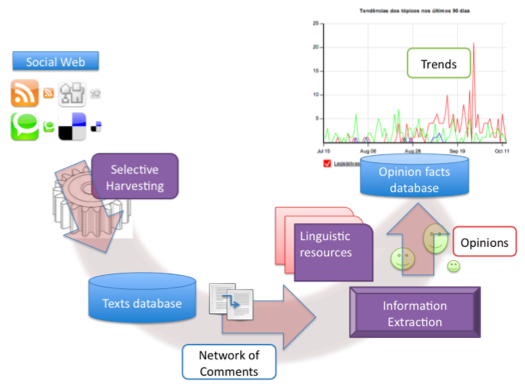
\includegraphics[width=.8\textwidth]{POPSTAR-bigpic}
\end{center}

\end{block}

\end{frame} 




\begin{frame} \frametitle{POPSTAR} 


\url{http://popstar.pt}

\begin{center}
     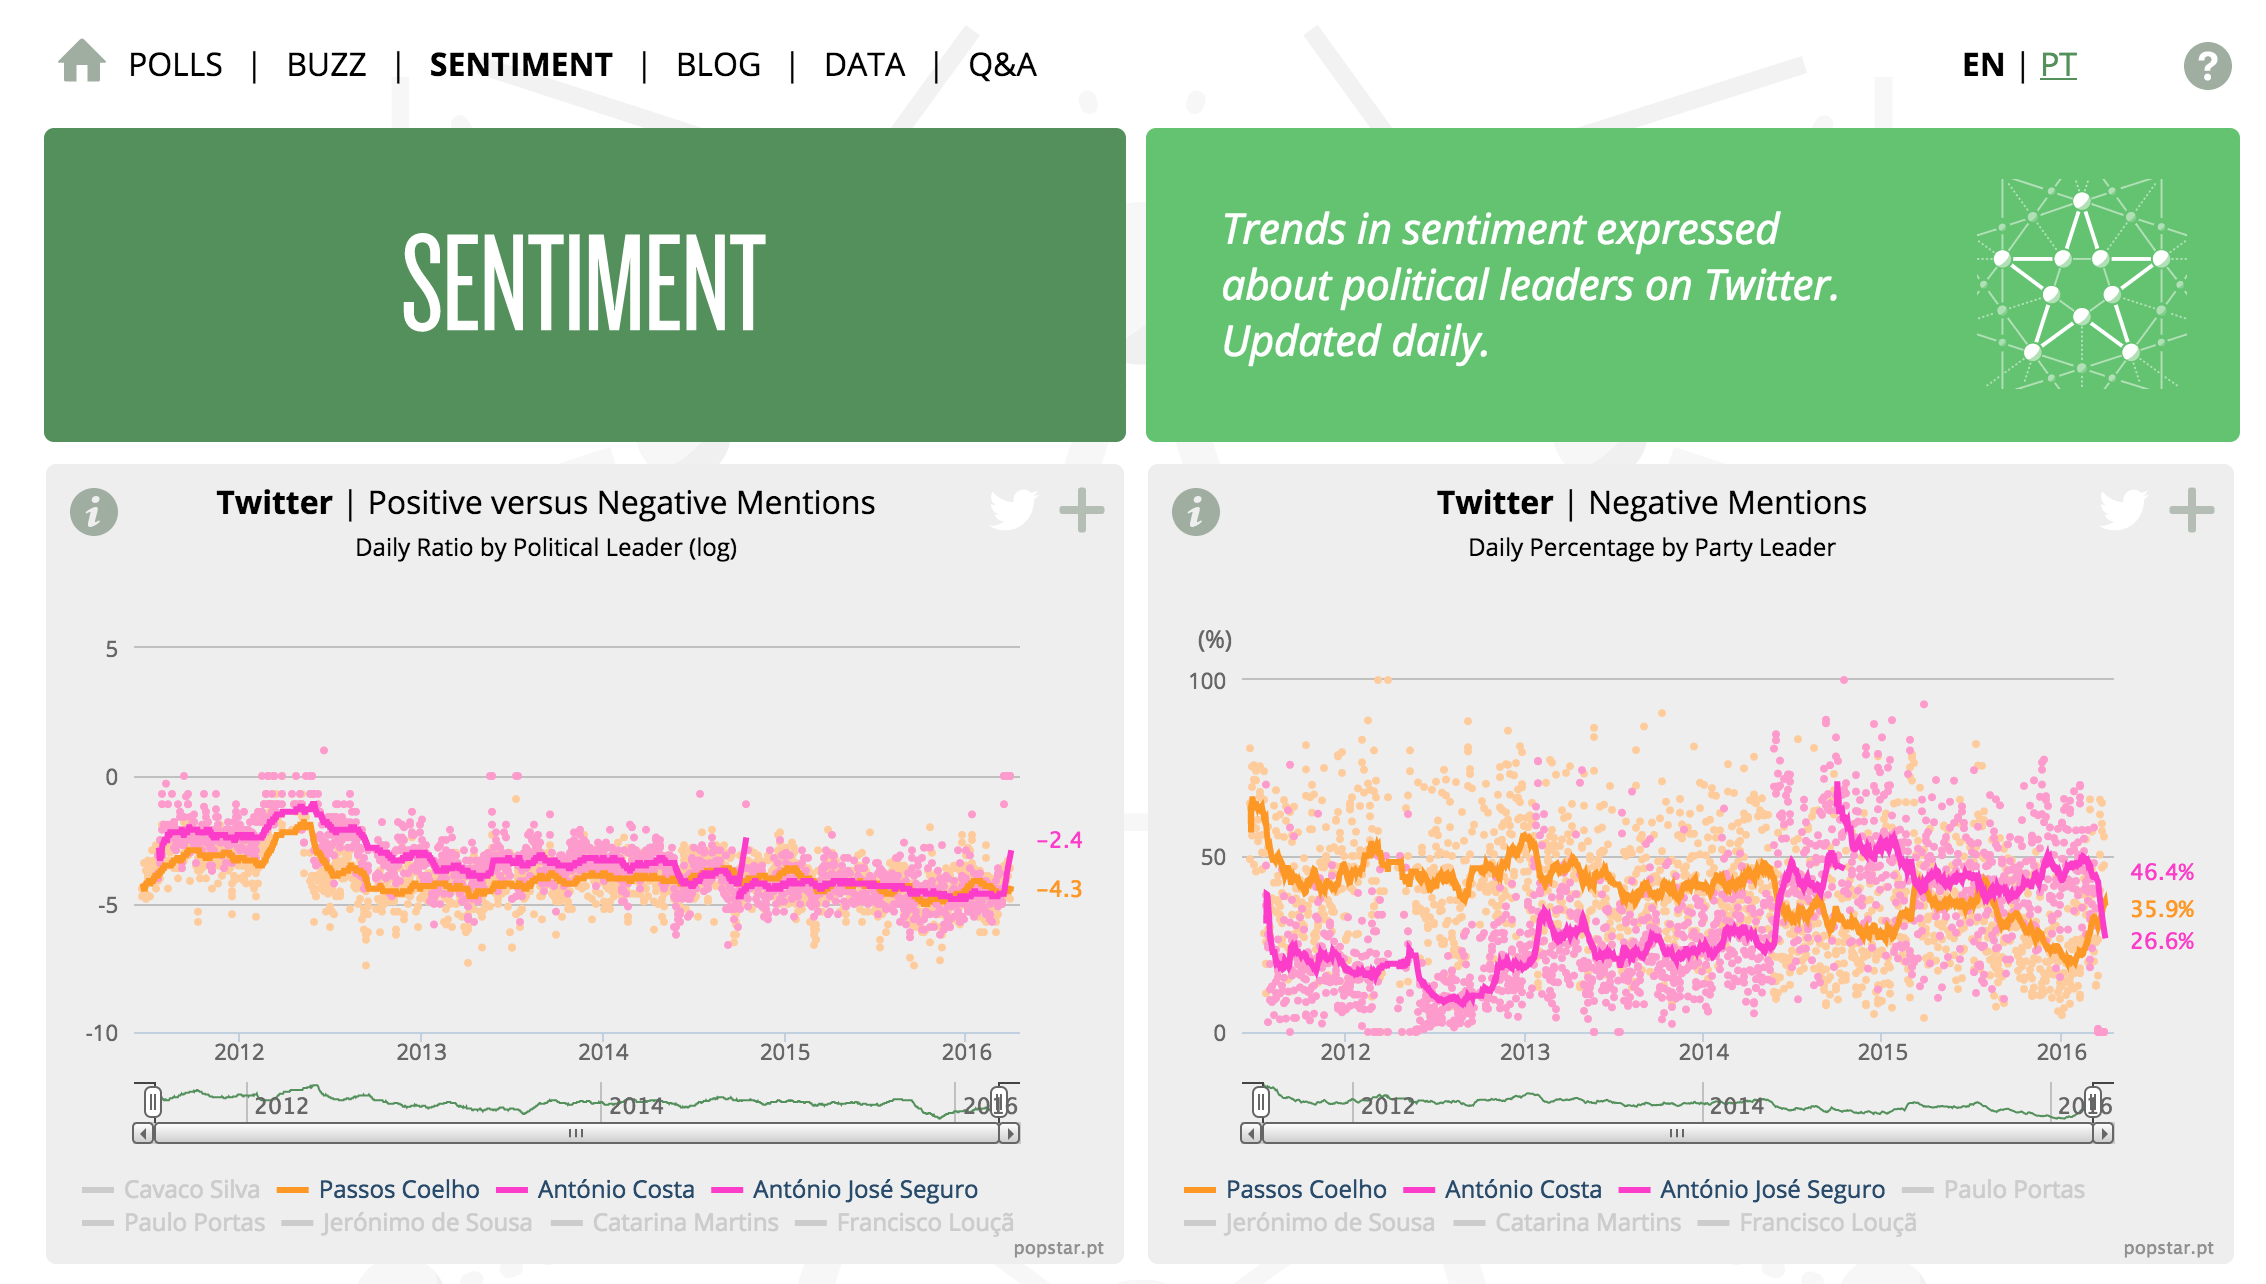
\includegraphics[width=.9\textwidth]{POPSTAR-screenshot}
\end{center}



\end{frame} 

\section{Opinion mining problem}

\begin{frame} \frametitle{Opinion Mining or Sentiment Analysis} %% BL2

\begin{block}{}

Computational study of opinions, sentiments, subjectivity, evaluations, attitudes, appraisal, affects, views, emotions, etc., expressed in text.

\begin{itemize}
\item Reviews, 
\item blogs, 
\item discussions, 
\item news, 
\item comments, 
\item feedback, 
\item or any other documents
\end{itemize}

\end{block}

\end{frame} 




\begin{frame} \frametitle{Opinion Mining Research \& Applications} %% BL6

\begin{itemize}

\item A popular research topic in NLP, text mining, and Web mining in recent
years.

%\begin{itemize}
%\item edited book:  (Shanahan, Qu, and Wiebe, 2006);
%\item surveys: (Pang and Lee 2008; Liu, 2006 and 2011; 2010)
%\end{itemize}

\item It has spread from computer science to management science 
% (Hu, Pavlou, Zhang, 2006; Archak, Ghose, Ipeirotis, 2007; Liu Y, et
% al 2007; Park, Lee, Han, 2007; Dellarocas, Zhang, Awad, 2007; Chen \& Xie 2007).

%40-60 companies in USA alone.

\item It touches every aspect of NLP and yet is confined. \\Little research in NLP/Linguistics in the past. 

\item Potentially a major technology from NLP. \\But it is hard

\end{itemize}
\end{frame} 


\begin{frame} \frametitle{Names \& Tasks} %% BL7 A large research area

Many names and tasks with somewhat different objectives and models
       
\begin{itemize}
\item Sentiment analysis 
\item  Opinion mining 
\item  Sentiment mining 
\item  Subjectivity analysis 
\item  Affect analysis 
\item  Emotion detection 
\item  Opinion spam detection 
\item  Etc.
\end{itemize}

\begin{block}{Sentiment Analysis or Opinion Mining?}
Sentiment analysis is more widely used in industry. \\
Both are widely used in academia, but they can be used interchangeably.
\end{block}

\end{frame} 



\begin{frame} \frametitle{Architecture of a Sentiment Analysis System} %% fm Feldman's review at CACM Apr 2013.

\begin{block}{Information Flow} 

\begin{center}
     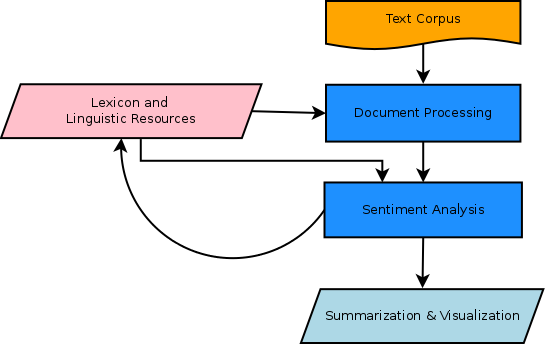
\includegraphics[width=\textwidth]{sentiment-analysis-flow}
\end{center}

\end{block}

\end{frame}


\begin{frame} \frametitle{Formulating the Opinion Mining Problem} %% BL 11

 %(Hu and Liu 2004)

\begin{block}{Abstraction 1: Opinion definition. What is an opinion? }

Can we provide a structured definition? \\
If we cannot structure a problem, we probably do not understand the problem.

\end{block}

\begin{block}{Abstraction 2: Opinion summarization: Why?} 

Opinions are subjective. An opinion from a single person (unless a VIP) is often not sufficient for action. \\
We need opinions from many people, and thus opinion summarization.

\end{block}

\end{frame} 



\begin{frame} \frametitle{Abstraction 1: What is an Opinion?}

% entities=red
% aspects=blue
% holders=brown

\begin{block}{Id: \textcolor{brown}{Abc123} on 5-1-2008} 
  ``I bought an \textcolor{red}{iPhone} a few days ago. It is such a
  nice \textcolor{blue}{phone}. The touch screen is really cool. The
  voice quality is clear too. It is much better than my old
  \textcolor{red}{Blackberry}, which was a terrible
  \textcolor{blue}{phone} and so difficult to type with its tiny
  \textcolor{blue}{keys}. However, \textcolor{brown}{my mother} was
  mad with me as I did not tell her before I bought the phone. She
  also thought the phone was too \textcolor{blue}{expensive}, ...''
\end{block}

One can \textbf{annotate} this review/blog at different levels:
\begin{description}  
\item [document level:]  is this review + or -? 
\item [sentence level:]  is each sentence + or -? 
\item [entity and aspect (feature) level:] is each aspect + or -?
 \end{description}

\end{frame} 


\begin{frame} \frametitle{Entity and Aspect Level}

\begin{block}{Id: \textcolor{brown}{Abc123} on 5-1-2008} 
  ``I bought an \textcolor{red}{iPhone} a few days ago. It is such a
  nice \textcolor{blue}{phone}. The touch screen is really cool. The
  voice quality is clear too. It is much better than my old
  \textcolor{red}{Blackberry}, which was a terrible
  \textcolor{blue}{phone} and so difficult to type with its tiny
  \textcolor{blue}{keys}. However, \textcolor{brown}{my mother} was
  mad with me as I did not tell her before I bought the phone. She
  also thought the phone was too \textcolor{blue}{expensive}, ...''
\end{block}

What do we see?
\begin{description}

\item [Opinion targets:] \textcolor{red}{entities} and their \textcolor{blue}{aspects} 
\item [Sentiments:] positive and negative 
\item [Opinion holders:] \textcolor{brown}{persons who hold the opinions}
\item [Time:] when opinions are expressed

\end{description}

\end{frame} 



\begin{frame} \frametitle{Two Main Types of Opinions} %% BL14

% (Jindal \& Liu 2006; Liu, 2010)

\begin{description}
\item [Regular opinions:] Sentiment/opinion expressions on some target entities

\begin{description}
\item [Direct opinions:] ``The touch screen is really cool.'' 
\item [Indirect opinions:] ``After taking the drug, my pain has gone.''
\end{description}

\item [Comparative opinions: ] Comparisons of more than one entity.
\begin{itemize}
\item E.g., ``iPhone is better than Blackberry.''
\end{itemize}

\item We focus on regular opinions first, and just call them opinions.

\end{description}

\end{frame} 



\begin{frame} \frametitle{A Restricted Definition of Opinion} %% BL 15

\begin{block}{Definition: (regular) opinion }

  An opinion (or regular opinion) is simply a \textcolor{green}{positive}
    or \textcolor{red}{negative} sentiment, view, attitude, emotion, or appraisal
  about an \textcolor{blue}{entity or an aspect of the entity}
% (Hu and Liu 2004; Liu 2006) 
from an \textcolor{brown}{opinion holder}
% (Bethard et al 2004; Kim and Hovy 2004; Wiebe et al 2005).

\end{block}

\begin{block}{Sentiment orientation of an opinion}

\begin{itemize}
\item positive, 
\item negative
\item neutral (no opinion)
\end{itemize}
Also called opinion orientation, semantic orientation, sentiment polarity.

\end{block}


\end{frame} 


\begin{frame} \frametitle{Entity and Aspect } %% BL16

%(Hu and Liu, 2004; Liu, 2006)

\begin{block}{Definition: entity} 

An entity $e$ is a product, person, event,organization, or topic. \\

$e$ is represented as a hierarchy of components, sub-components, and
so on. Each node represents a component and is associated with a set
of attributes of the component. 

\end{block}

\begin{block}{Definition: aspect} 

An opinion can be expressed on any node or attribute of the node. \\

{\em aspects (features)} designate both components and attributes.

\end{block}

\end{frame} 


\begin{frame} \frametitle{A Definition of Opinion} %% BL17

An opinion is a quintuple 

\begin{equation*}
(e_j, a_{jk}, so_{ijkl}, h_i, t_l), 
\end{equation*}

where

\begin{itemize}
\item $e_j$ is a target entity. 
\item $a_{jk}$ is an aspect/feature of the entity $e_j$. 

\item $so_{ijkl}$ is the sentiment value of the opinion from the
  opinion holder $h_i$ on feature $a_{jk}$ of entity $e_j$ at time
  $t_l$.  

\item $so_{ijkl}$ is +ve, -ve, or neu, or more granular ratings. 
\item $h_i$ is an opinion holder. 
\item $t_l$ is the time when the opinion is expressed.
\end{itemize}

\small{(Liu, Chapter in NLP handbook, 2010)}


\end{frame} 


\begin{frame} \frametitle{Some Remarks about the Definition} %% BL18

\begin{itemize}

\item Although introduced using a product review, the definition is
  generic \\
Applicable to other domains, like politics, social events, services,
topics, etc. 

\item $(e_j, a_{jk})$ is also called the \textbf{opinion target} \\
An opinion without knowing the target is of limited use.


\item The five components in $(e_j, a_{jk}, so_{ijkl}$, $h_i$, $t_l$)
  must correspond to one another. Very hard to achieve. 

\item The five components are essential. Without any of them, it can be problematic in general.


\end{itemize}

\end{frame} 


\begin{comment}

\begin{frame} \frametitle{Some Remarks about the Definition (cont.)} %% BL19


\begin{itemize}
\item Of course, one can add any number of other components to the
  tuple for more analysis. E.g., \\
Gender, age, Web site, post-id, etc.

\item The original definition of an entity is a hierarchy of parts, sub-parts, and so on.

\begin{itemize}

\item The simplification can result in information loss. \\

E.g., ``The seat of this car is rally ugly.'' ``seat'' is a part of the car and ``appearance'' (implied by ugly) is an aspect of ``seat'' (not the car).

\item But it is usually sufficient for practical applications. \\
It is too hard without the simplification.
\end{itemize}

\end{itemize}

\end{frame} 




\begin{frame} \frametitle{Confusing Terminologies} %% BL20

\begin{itemize}
\item Entity a.k.a. \textit{object}. 

\item Aspect a.ka. \textit{feature}, \textit{attribute}, \textit{facet}, etc 

\item Opinion holder is also called \textit{opinion source} 

\item \textit{topic} sometimes used as alternative name for entity and/or aspect.\\
Separating entity and aspect is preferable

\item Application/domain-specific terms: 
\begin{itemize}
   \item \textit{product features}, 
   \item \textit{political issues}, etc.
\end{itemize}

\end{itemize}

\end{frame} 

\end{comment} 


\begin{frame} \frametitle{Reader's Standing Point} %BL21

\begin{block}{ Consider this sentence:}
``I am so happy that Google price shot up today.''
\end{block}

\begin{itemize}
\item Although the sentence gives an explicit sentiment, different readers may feel very differently.

\begin{itemize}
    \item If a reader sold his Google shares yesterday, he will not be
  that happy. 
    \item If a reader bought a lot of Google shares yesterday, he will be very happy.
\end{itemize}

\item Current research either implicitly assumes a standing point, or ignores the issue.

\end{itemize}

\end{frame} 

\begin{frame} \frametitle{The Example Blog in Quintuples} %BL22

\begin{block}{Id: Abc123 on 5-1-2008 }
``I bought an iPhone a few days ago. It is such a nice phone. The touch screen is really cool. The voice quality is clear too. It is much better than my old Blackberry, which was a terrible phone and so difficult to type with its tiny keys. However, my mother was mad with me as I did not tell her before I bought the phone. She also thought the phone was too expensive, ...''
\end{block}

\begin{block}{In quintuples}

\begin{equation*}
(iPhone, GENERAL, +, Abc123, 5-1-2008) 
\end{equation*}

\begin{equation*}
 (iPhone, touch\_screen, +, Abc123, 5-1-2008) 
\end{equation*}
\end{block}

We will discuss comparative opinions later.
\end{frame} 

\begin{frame} \frametitle{Structure the Unstructured} %% BL23

\begin{itemize}

\item Objective: Given an opinionated document, \\
Discover all quintuples $(e_i, a_{jk}, so_{ijkl}, h_k, t_l)$, \\
Or, solve some simpler forms of the problem \\
\begin{itemize}
   \item E.g., sentiment classification at the document or sentence level.
\end{itemize}

\item With the quintuples, \\
Unstructured Text $\rightarrow$ Structured Data
\begin{itemize}
\item Traditional data and visualization tools can be used to slice,
  dice and visualize the results. 
\item Enable qualitative and quantitative analysis.
\end{itemize}


\end{itemize}

\end{frame} 


%%%% Emotion %%%%%%

\begin{comment}

\begin{frame} \frametitle{Subjectivity and Emotion} %% BL 24

Two closely related concepts. 

\begin{block}{Sentence subjectivity:} 

An objective sentence presents some factual information, while a
subjective sentence expresses some personal feelings, views, emotions,
or beliefs.  

\end{block}


\begin{block}{Emotion:} 

Emotions are people's subjective feelings and thoughts.

\end{block}

\end{frame} 


\begin{frame} \frametitle{Subjectivity} %% 25

\begin{columns}[T]

\begin{column}{0.50\textwidth}

Subjective expressions come in many forms \small{(Wiebe 2000; Wiebe et al 2004; Riloff et al 2006)}: \\
\begin{tabular}{l}
opinions, \\
allegations, \\
desires, \\
beliefs, \\
suspicions, \\
speculations 
\end{tabular} 

\begin{block}{}
{\bf A subjective sentence may contain a positive or negative opinion}
\end{block}
\
\end{column}

\begin{column}{0.45\textwidth}
Most opinionated sentences are subjective, but {\bf objective sentences can
imply opinions too} %\small{(Liu, 2010)}
\begin{itemize} 
\item ``The machine stopped working in the second day'' 
\item ``We brought the mattress yesterday, and a body impression has
  formed.'' 
\item ``After taking the drug, there is no more pain''
\end{itemize}

\end{column}

\end{columns}

\end{frame} 


\begin{frame} \frametitle{Emotion} %% BL 26

No agreed set of basic emotions of people among researchers. Based on
Parrott (2001), people have {\bf six main emotions},

\begin{tabular}{ll}
love & amor\\
joy & alegria\\ 
surprise & surpresa\\ 
anger &  ira \\
sadness & tristeza\\
fear & medo 
\end{tabular}

\begin{block}{}
Strengths of opinions/sentiments are related to certain emotions,
e.g., joy, anger. \\
However, {\bf the concepts of emotions and opinions are not equivalent.}
\end{block}

\end{frame} 


\begin{frame} \frametitle{Rational and Emotional Evaluations} % BL 27

\begin{columns}[T]


\begin{column}{.45\textwidth}
\begin{block}{Rational evaluation:} 
``The voice of this phone is clear''  \\
Many evaluation/opinion sentences express no emotion \\
\end{block}

\end{column}

\begin{column}{.45\textwidth}
\begin{block}{Emotional evaluation}
``I love this phone'' \\
``The voice of this phone is crystal clear'' (?)
 \end{block}
\end{column}

\end{columns}

\begin{block}{}
Some emotion sentences express no (positive or negative)
sentiment: \\
``I am so surprised to see you''.
\end{block}
\end{frame} 


\begin{frame} \frametitle{Sentiment, Subjectivity, and Emotion} %% BL28

Although they are clearly related, these concepts are not the same:  \\ 
\begin{center}
Sentiment  $\neq$ subjective $\neq$ emotion
\end{center}

\vfill
sentiment is not a subset of subjectivity (without implied sentiments by facts, it should be)  
\begin{center}
sentiment  $\not\subset$ subjectivity
\end{center}

\vfill
The following should hold:  
\begin{center}
emotion $\subset$ subjectivity  \\
sentiment $\not\subset$ emotion \\
\end{center}

\end{frame} 

\end{comment} 

%%%% End Emotion %%%%%%


\begin{frame} \frametitle{Abstraction 2: Opinion Summary} %%29


\colorbox{yellow}{\parbox{0.9 \textwidth} {\textbf{A multi-document summarization task}}}

\vfill
For factual texts, summarization is to select the most important facts
and present them in a sensible order while avoiding repetition \\
\begin{itemize}
\item 1 fact $=$ any number of the same fact
\end{itemize}

\vfill
For opinion documents, it is different:  opinions have a quantitative side \& have targets
 \begin{itemize}
\item 1 opinion  $\ne$ a number of opinions \\
\item Aspect-based summary is more suitable 
\end{itemize}

\vfill
\colorbox{yellow}{\parbox{0.9 \textwidth} {\textbf{Quintuples form the basis for opinion summarization}}}

\end{frame} 

\begin{frame} \frametitle{Aspect-based Opinion Summary} %% BL30


 \begin{columns}[T]

\begin{column}{0.38\textwidth}

\begin{block}{Review of iPhone:}
\small{
``I bought an iPhone a few days
ago. It is such a nice phone. The touch screen is really cool. The voice quality is clear too. It is much better than my old Blackberry, which was a terrible phone and so difficult to type with its tiny keys. However, my mother was mad with me as I did not tell her before I bought the phone. She also thought the phone was too expensive, ..''}
\end{block}


\end{column}

\begin{column}{0.58\textwidth}

\begin{block}{Aspect 1: Touch screen}

\begin{description}
\item [Positive:] 212
\end{description}

\small{The touch screen was really cool.  \\
The touch screen was so easy to use ... \\}

\begin{description}
\item [Negative:] 6 
\end{description}

\small{The screen is easily scratched. \\
I have a lot of difficulty in removing finger marks from the  touch
screen. ... }

\end{block}

\begin{block}{Aspect 2: voice quality}
... 
\end{block}

Note: We omit opinion holders

    \end{column}
\end{columns}


\end{frame} 




\begin{frame} \frametitle{Visualization of Aspect-based Summaries} %% 31


\begin{block}{Opinion Observer} % (Liu et al. 2005) 

\begin{center}
     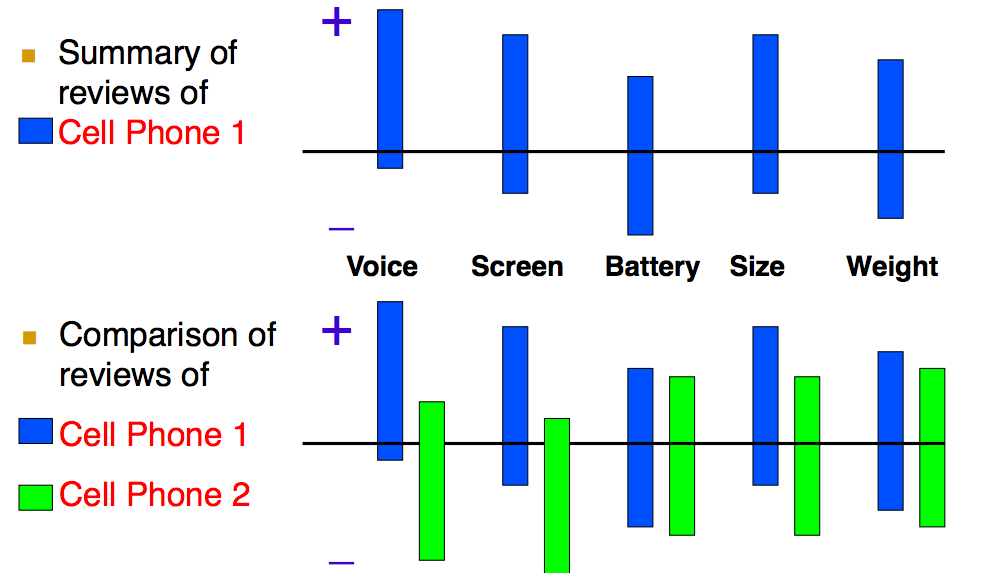
\includegraphics[width=\textwidth]{opinion-observer}
\end{center}

\end{block}

\end{frame} 


\begin{comment} 

\begin{frame} \frametitle{Visualization of Aspect-based Summaries} %% 32


\begin{block}{Bing} 

\begin{center}
     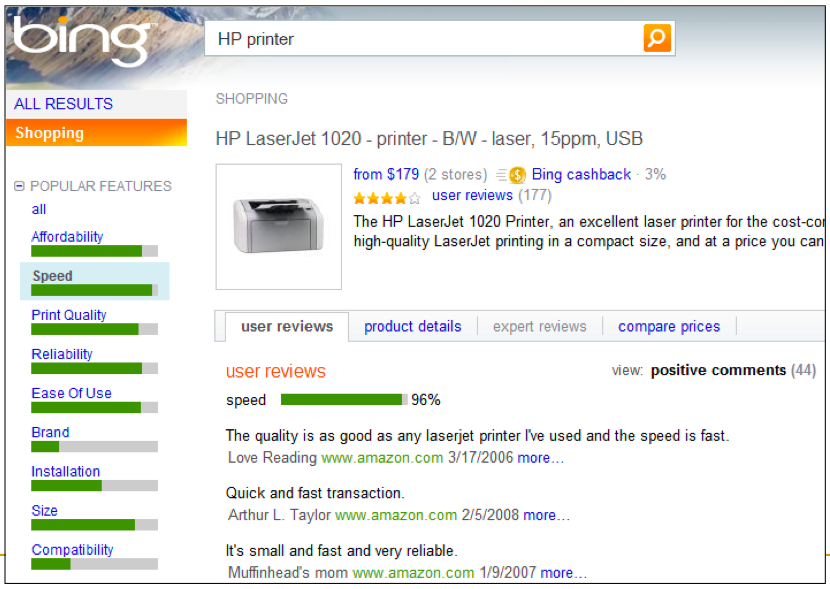
\includegraphics[width=0.85\textwidth]{bing-shopping}
\end{center}
\end{block}


\end{frame} 

\begin{frame} \frametitle{Visualization of Aspect-based Summaries} %%33


\begin{block}{Google Product Search (Blair-Goldensohn et al 2008) \url{http://www.google.com/shopping}} 

\begin{center}
     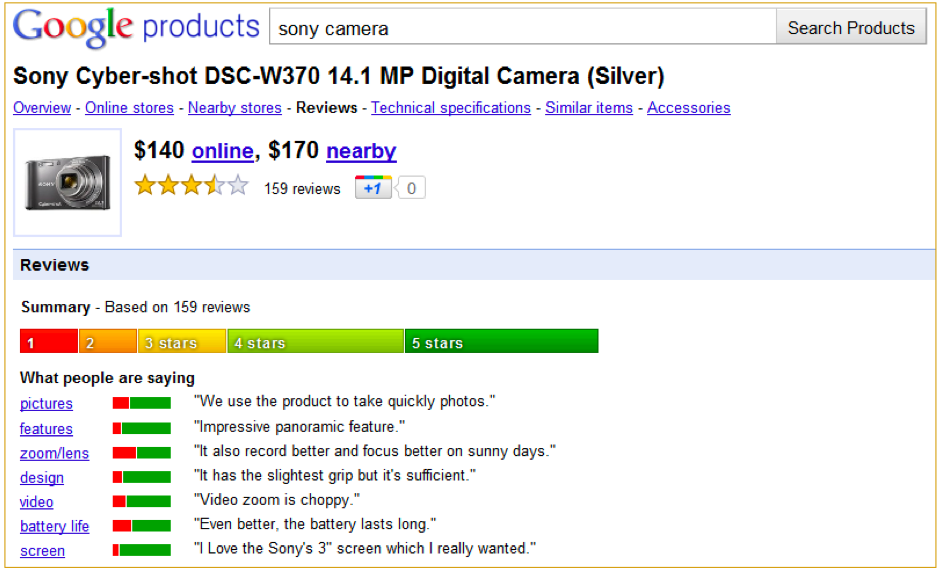
\includegraphics[width=\textwidth]{google-product-search}
\end{center}
\end{block}

\end{frame} 

\end{comment} 

\begin{frame} \frametitle{Visualization of Aspect-based Summaries} %%33bis


\begin{block}{} %% Booking

\begin{center}
     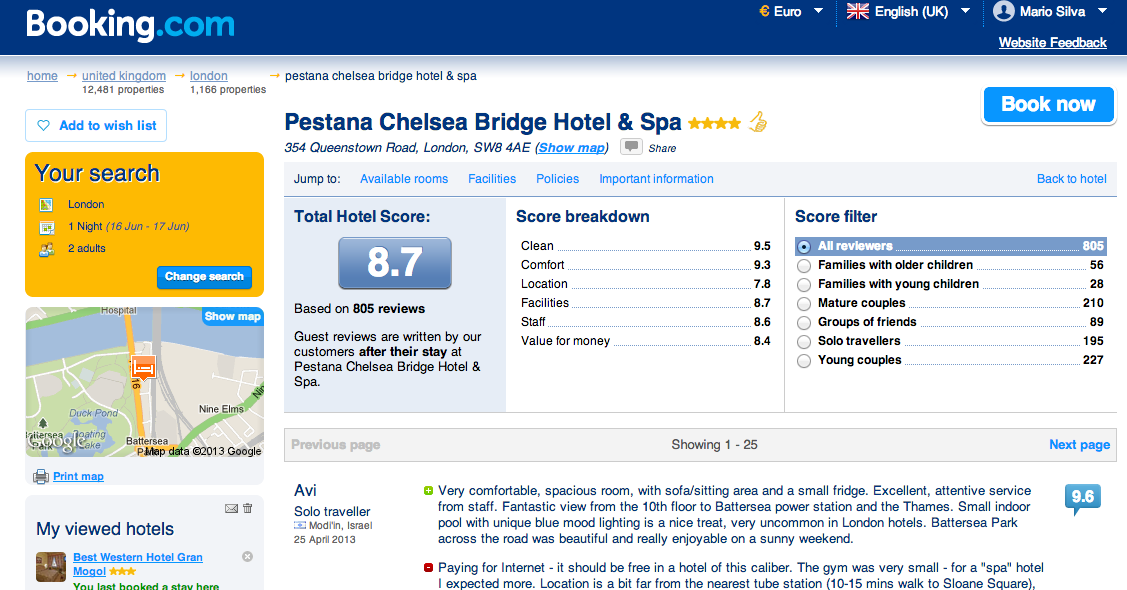
\includegraphics[width=\textwidth]{booking-aspect-summary}
\end{center}
\end{block}

\end{frame} 



%% \begin{frame} \frametitle{Some Examples of Opinion EQ} %% 34 
%% \end{frame} 


\begin{frame} \frametitle{Detail opinion sentences} %%35 - merkel


\begin{block}{\url{http://pattie.fe.up.pt/sentibubbles/merkel/}} 

\begin{center}
     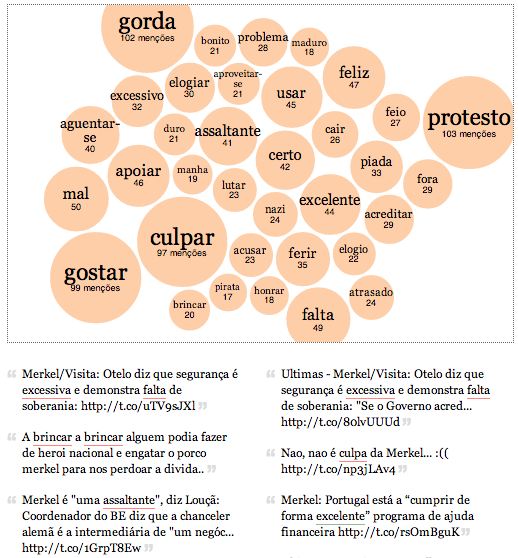
\includegraphics[width=\textwidth]{sentibubbles}
\end{center}

\end{block}


\end{frame} 

%%\begin{frame} \frametitle{\% of +ve opinion and # of opinions} %% 36
%% \end{frame} 


\begin{frame} \frametitle{Aggregate Opinion Trends} %%37

\begin{block}{\url{http://legislativas.sapo.pt/2011/twitometro/}} 

\begin{center}
     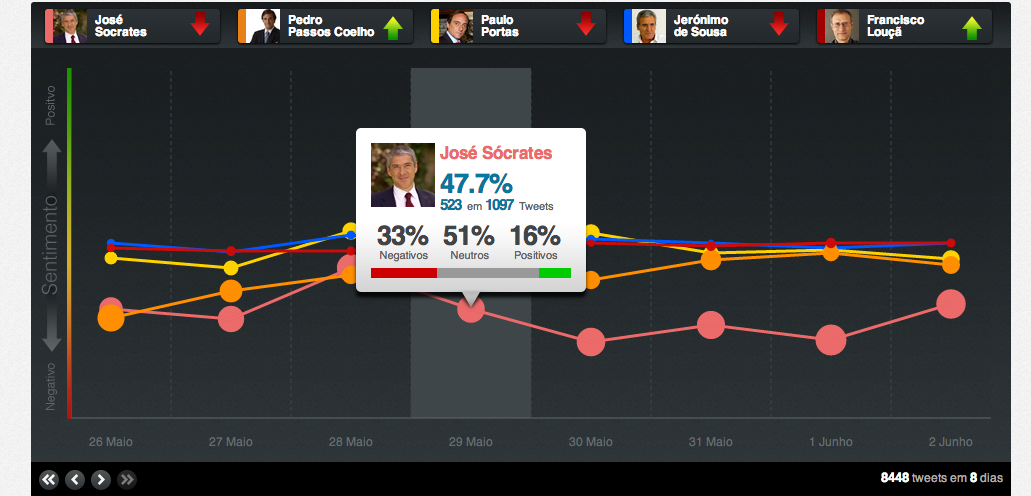
\includegraphics[width=\textwidth]{twitometro}
\end{center}

\end{block}

\end{frame} 



%% 38 \begin{frame} \frametitle{} \end{frame} 

\begin{frame} \frametitle{Five Pieces of Information Must Match} %%39

\begin{equation*}
(e_j, a_{jk}, so_{ijkl}, h_i, t_l)     
\end{equation*}

\begin{description}
\item [$e_j$]  a target entity: Named Entity Extraction (more) 
\item [$a_{jk}$] an aspect of ej: Information Extraction 
\item [$so_{ijkl}$] is sentiment: Sentiment Identification 
\item [$h_i$] is an opinion holder: Information/Data Extraction 
\item [$t_l$] is the time: Information/Data Extraction 
\end{description}


Coreference resolution 

Synonym match (voice = sound quality) ...


\end{frame} 


\begin{frame} \frametitle{Opinion Mining is Hard!} %%40

\begin{block}{}
``This past Saturday, I bought a Nokia phone and my girlfriend bought a
Motorola phone with Bluetooth. We called each other when we got
home. The voice on my phone was not so clear, worse than my previous
Samsung phone. The battery life was short too. My girlfriend was quite
happy with her phone. I wanted a phone with good sound quality. So my
purchase was a real disappointment. I returned the phone yesterday.''
\end{block}

\end{frame} 


\begin{frame} \frametitle{Opinion Mining: Easier and Harder Problems} %% 41

\begin{columns}[T]

\begin{column}{0.5 \textwidth}

\begin{enumerate}

\item Tweets are the easiest \\
\textbf{short and thus usually straight to the point} 

\item Reviews are next\\
\textbf{entities are given (almost) and there is little noise} 

\item Discussions, comments, and blogs are hard.\\
\textbf{Multiple entities, comparisons, noisy, \textcolor{blue}{sarcasm}, etc}
\end{enumerate}

\end{column}

\begin{column}{0.5 \textwidth}

\begin{block}{}
\begin{itemize}
\item Determining sentiments seems to be easier. 
\item Extracting entities and aspects is harder. 
\item Combining them is even harder.
\end{itemize}
\end{block}

\end{column}

\end{columns}
\end{frame} 


\begin{frame} \frametitle{Opinion Mining: Process Steps} %% 42

\begin{enumerate}

\item Source the data, e.g., reviews, blogs, etc
   \begin{itemize}
      \item Crawl all data, store and search them, or 
      \item Crawl only the target data
   \end{itemize}

\item Extract the right entities \& aspects
\begin{itemize}
\item Group entity and aspect expressions, \\  Moto = Motorola, photo = picture, etc ...

\end{itemize}

\item Aspect-based opinion mining (sentiment analysis)
\begin{itemize}
\item Discover all quintuples \\
(Store the quintuples in a database)
\end{itemize}

\item Aspect based opinion summary

\end{enumerate}


\end{frame} 


\begin{comment} 

\begin{frame} \frametitle{Opinion Mining Tasks} 

\begin{block}{At the document (or review) level:}
\begin{itemize}
\item \textbf{Task:} Sentiment classification of reviews \\
Classes: positive, negative, and neutral \\
Assumption: each document (or review) focuses on a single entity (not
true in many discussion posts) and contains opinion from a single
opinion holder.
\end{itemize}

\end{block}

\begin{block}{At the sentence level:}
\begin{itemize}
\item \textbf{Task 1:} identifying subjective/opinionated sentences \\
Classes: objective and subjective (opinionated)

\item\textbf{Task 2:} sentiment classification of sentences \\
Classes: positive, negative and neutral. \\
Assumption: a sentence contains only one opinion not true in many cases. 
Then we can also consider clauses or phrases.

\end{itemize}

\end{block}

\end{frame}

\begin{frame} \frametitle{Opinion Mining Tasks (cont.)} 

\begin{block}{At the aspect level:}
\begin{itemize}
\item \textbf{Task 1 (entity extraction and grouping):} Extract all
  entity expressions, and group synonymous entity expressions into
  entity clusters. \\
  Each cluster indicates a unique entity $e_i$.

\item \textbf{Task 2 (aspect extraction and grouping):} Extract all
  aspect expressions of the entities, and group synonymous aspect
  expressions into clusters. \\
  Each aspect expression cluster of entity
  $e_i$ indicates a unique aspect $a_{ij}$.  

\end{itemize}

\end{block}

\end{frame}

\begin{frame} \frametitle{Opinion Mining Tasks (cont.)} 

\begin{block}{}
\begin{itemize}
\item \textbf{Task 3 (opinion holder and time extraction):} Extract these pieces of information from the text or structured data.
\item \textbf{Task 4 (aspect sentiment classification):} Determine whether each opinion on an aspect is positive, negative or neutral. 
\item \textbf{Task 5 (opinion quintuple generation):} Produce all opinion quintuples $(e_i, a_{ij}, so_{ijkl}, h_k, t_l)$,  expressed in $D$. 

\end{itemize}

\end{block}

\end{frame}

\end{comment} 



\section{Document sentiment classification}


\begin{frame} \frametitle{Sentiment Classification} %%44

\begin{block}{Task:}
Classify a whole opinion document (e.g., a review) based on the
\textbf{overall sentiment of the opinion holder} \\ 
%\small{(Pang et al 2002; Turney 2002)}
 
\vfill
\textbf{Classes:} Positive, negative (possibly neutral) \\
 Neutral or no opinion is hard. Most papers ignore it. 
\end{block}

\begin{block}{An example review:}

``I bought an iPhone a few days
ago. It is such a nice phone, although a little large. The touch
screen is cool. The voice quality is clear too. I simply love it!'' 

\textbf{Classification:} \textcolor{green}{positive} or \textcolor{red}{negative}?

\end{block}


\colorbox{yellow}{\parbox{0.9 \textwidth} {\textbf{The most widely studied problem.}}}



\end{frame} 


\begin{frame} \frametitle{Opinion Mining as a Text Classification Task} %%45
 

A text classification problem, but different from topic-based text
classification. 

In topic-based text classification (e.g., computer, sport, science),
topic words are important. 

\vfill

In sentiment classification, \textcolor{red}{{\bf opinion/sentiment words}} are more
important: 

\begin{columns}

\begin{column}{0.5 \textwidth}

\begin{center}
\begin{tabular}{l}
great, \\
excellent, \\
horrible, \\
bad, \\
worst, \\
etc. 
\end{tabular}
\end{center}

\end{column}

\begin{column}{0.5 \textwidth}

\fcolorbox{red}{white}{\parbox{0.9 \textwidth}{\textbf{Opinion/sentiment words:} 
words/phrases that express desired or undesired states or qualities.}
}

\end{column}
\end{columns}


\end{frame} 

\begin{frame} \frametitle{Opinion Mining as Text Classification} %%46

\begin{columns}[T]

\begin{column}{.40\textwidth}

\begin{block}{Assumption:} 

{\large The text is written by a single author and expresses sentiment
  on a single entity.}

\end{block}

\begin{block}{Goal:} 

{\large
discover $so$   

$(\_, \ _, so,\_, \_)$
}

$e$, $a$, $h$, and $t$ are ignored
\end{block}

\end{column}

\begin{column}{.55\textwidth}


\fcolorbox{red}{white}{\parbox{\textwidth}{\textbf{Compliance with Assumption:} 

\begin{itemize}
\item Reviews usually satisfy it: \\
Most research work uses reviews. \\
Author ranked: Positive: 4 or 5 stars, negative: 1 or 2 stars 

\item Many forum postings and blogs do not: \\
They can mention and compare multiple entities \\
Many postings express no sentiment
\end{itemize}
}}

\end{column}

\end{columns}

\end{frame} 




\begin{frame} \frametitle{A Review (amazon.com)} %%47

\begin{block}{\url{http://tinyurl.com/cndq5jl}} 

\begin{center}
     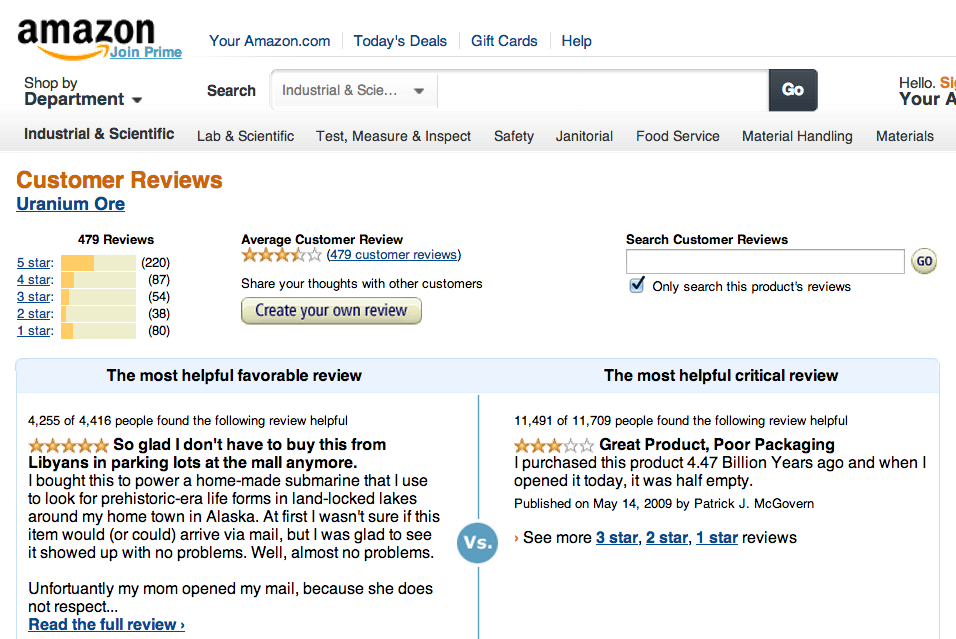
\includegraphics[width=\textwidth]{amazon-review}
\end{center}

\end{block}

\end{frame} 




\begin{frame} \frametitle{A Review (imdb.com)} %%47

\begin{block}{\url{http://tinyurl.com/cndq5jl}} 

\begin{center}
     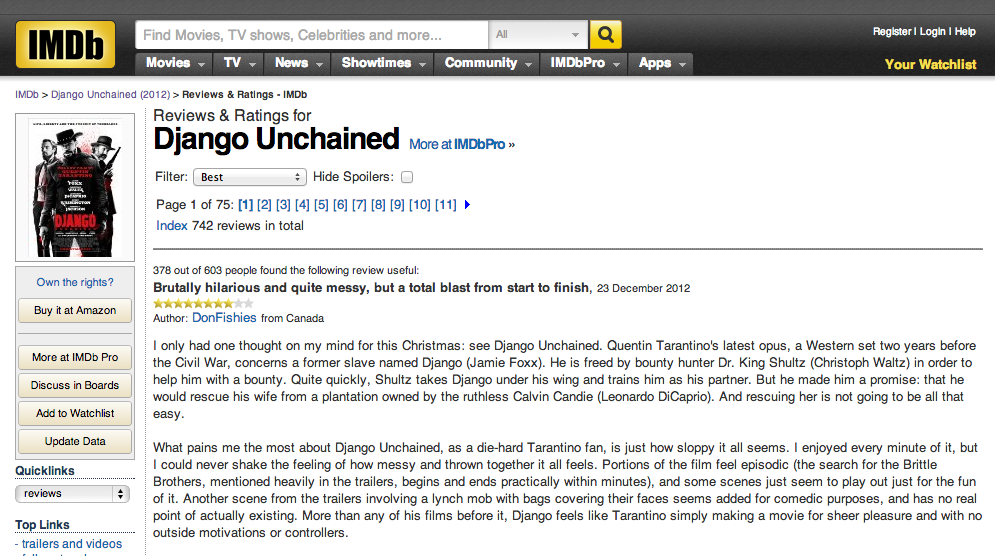
\includegraphics[width=\textwidth]{imdb-review}
\end{center}

\end{block}


\end{frame} 



\begin{frame} \frametitle{A Review (fnac.pt)} %%47

\begin{block}{\url{http://tinyurl.com/cp9avtr}} 


\begin{center}
     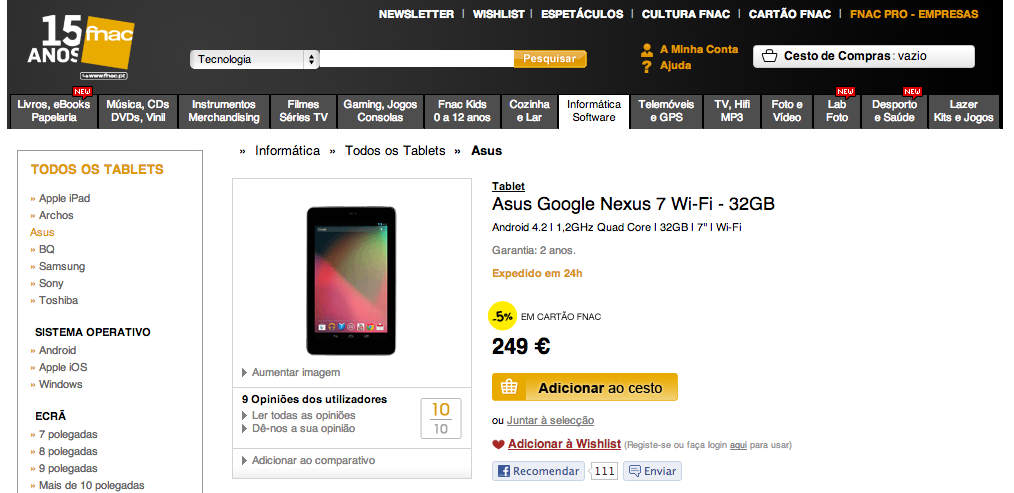
\includegraphics[width=0.3\textwidth]{fnac-review1}
\end{center}

\begin{center}
     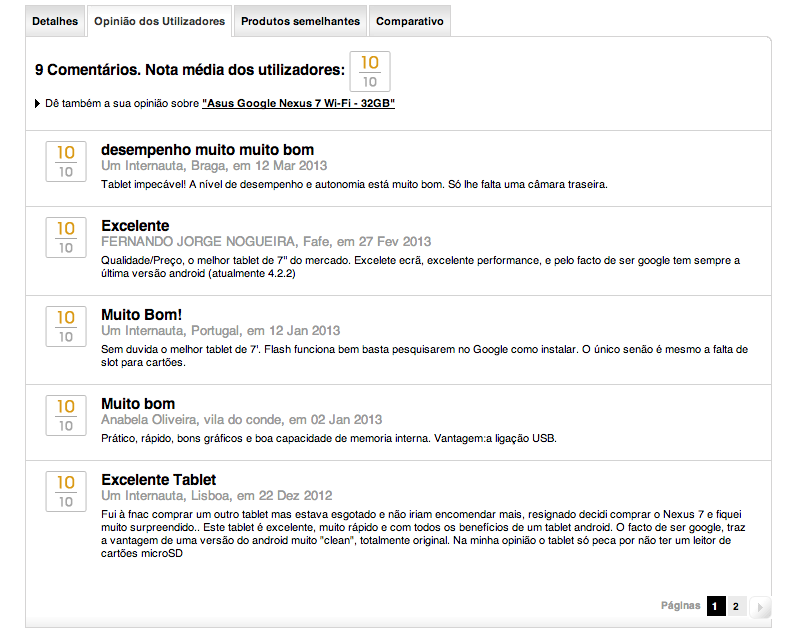
\includegraphics[width=\textwidth]{fnac-review2}
\end{center}

\end{block}


\end{frame} 


\begin{frame} \frametitle{Unsupervised Classification} %%48


\fcolorbox{red}{white}{\parbox{0.9 \textwidth}{
    (Turney, 2002): ``Thumbs
    Up or Thumbs Down? Semantic Orientation Applied to Unsupervised
    Classification of Reviews'' \\
   \url{http://acl.ldc.upenn.edu/P/P02/P02-1053.pdf}
}}

\vfill

\textbf{Data:} reviews from {\tt epinions.com} on automobiles, banks, movies, and
travel destinations. 

\vfill

Three-step approach:
\begin{enumerate}
\item Extract patterns with Part-of-Speech (POS) tags

\item Estimate Semantic Orientation (SO) of each pattern

\item Compute average SO of the review

\end{enumerate}

\end{frame} 


\begin{frame}[fragile]

 \frametitle{Part-of-speech (POS) Tagging}

 
\begin{block}{Available in NLTK!}
{\small
\begin{verbatim} 	
>>> text = nltk.word_tokenize("They refuse to permit us to
           obtain the refuse permit")
>>> nltk.pos_tag(text)
[('They', 'PRP'), ('refuse', 'VBP'), ('to', 'TO'), 
('permit', 'VB'), ('us', 'PRP'),
('to', 'TO'), ('obtain', 'VB'), ('the', 'DT'), 
('refuse', 'NN'), ('permit', 'NN')]
\end{verbatim}
}
\end{block}

See Penn Treebank POS Tags: \url{http://www.ling.upenn.edu/courses/Fall_2003/ling001/penn_treebank_pos.html}


\end{frame} 


\begin{frame} \frametitle{ Step 1: Patterns of POS tags} %%49

Extract two consecutive words (two-word phrases) from reviews if their
tags conform to a pattern

\begin{center}
     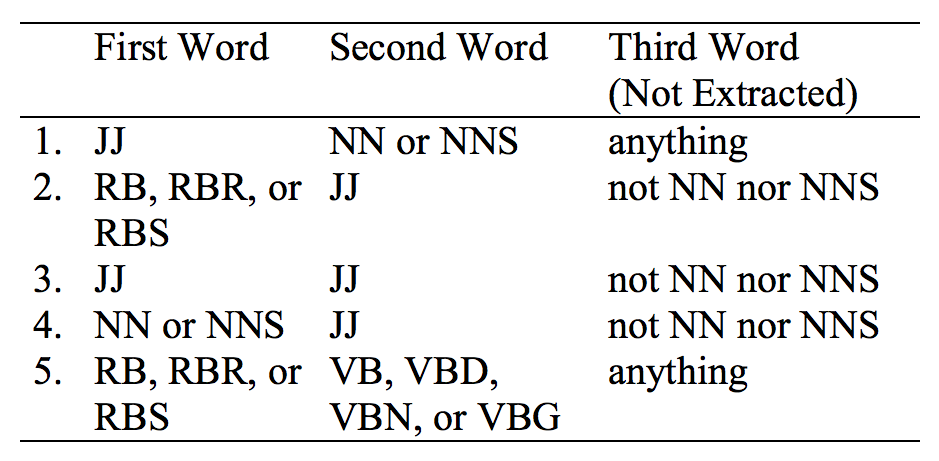
\includegraphics[width=\textwidth]{turney01}
\end{center}

\end{frame} 

\begin{frame} \frametitle{Pointwise Mutual Information}

%% P ( word1  word 2 )  PMI ( word1 , word 2 ) = log 2    P ( word ) P ( word )  1 2  
\begin{center}
     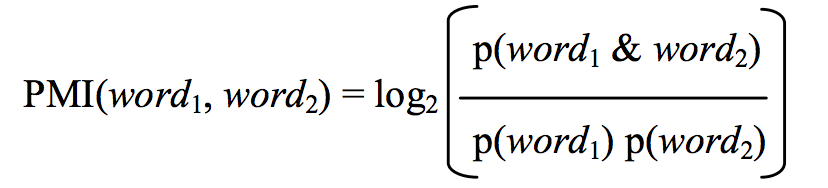
\includegraphics[width=.8\textwidth]{turney02}
\end{center}

\vfill

\begin{center}
\small{
The PMI of a pair of outcomes $x$ and $y$ belonging to discrete random
variables $X$ and $Y$ quantifies the discrepancy between the probability
of their coincidence given their joint distribution and their
individual distributions, \textbf{assuming independence}. } \\

\begin{equation*}
PMI(x,y) = log \frac{p(x,y)}{p(x)p(y)}
\end{equation*}

\tiny{\url{http://en.wikipedia.org/wiki/Pointwise_mutual_information}}
\end{center}
\end{frame}

\begin{frame} \frametitle{Step 2: Estimate the SO of each Phrase} %% 50


Semantic orientation (SO):
%% SO(phrase) = PMI(phrase, ``excellent'') - PMI(phrase, ``poor'')

\begin{center}
     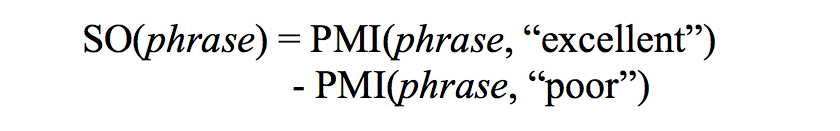
\includegraphics[width=0.8\textwidth]{turney03}
\end{center}

Altavista search to find the number of hits to compute PMI and SO.

\begin{center}
     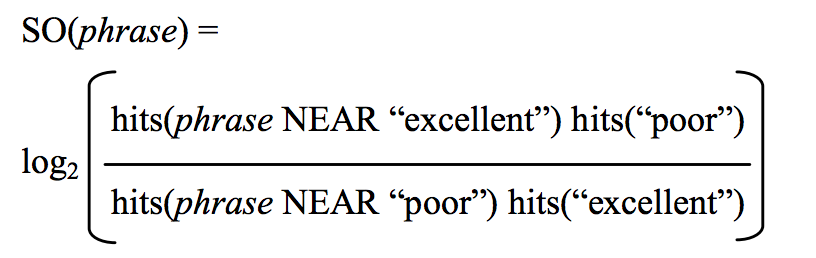
\includegraphics[width=0.8 \textwidth]{turney04}
\end{center}

\end{frame} 

\begin{frame} \frametitle{Step 3: Compute the Average SO of All
    Phrases} %% 51

Classify the review as:
\begin{itemize}
\item positive, if average SO is positive, 
\item negative otherwise.
\end{itemize}

\vfill
Final classification accuracy: \\
\begin{tabular}{l l}
automobiles & 84\% \\
banks & 80\% \\
movies & 65.83\% \\
travel destinations & 70.53\%
\end{tabular}

\end{frame} 



\begin{frame} \frametitle{A Positive Review}
\begin{center}
     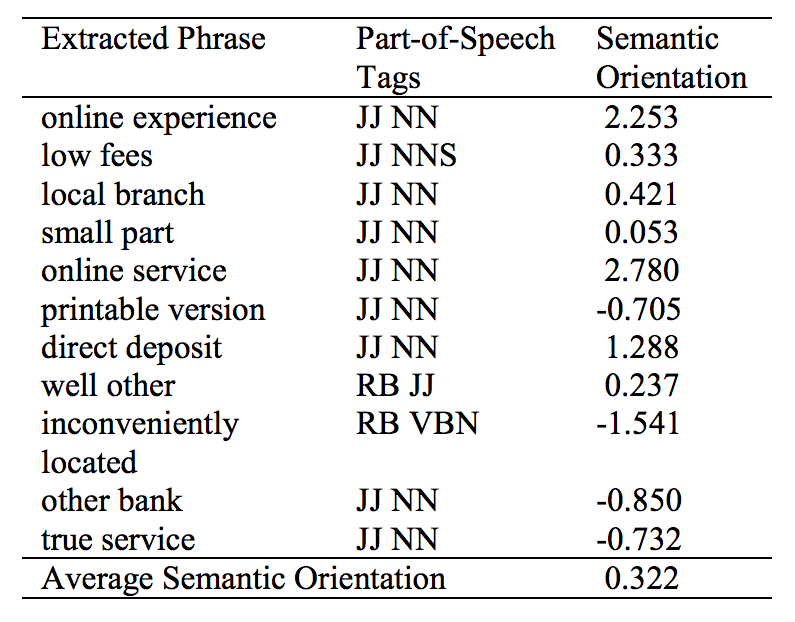
\includegraphics[width=0.9\textwidth]{turney05}
\end{center}
\end{frame} 


\begin{frame} \frametitle{A Negative Review}

\begin{center}
     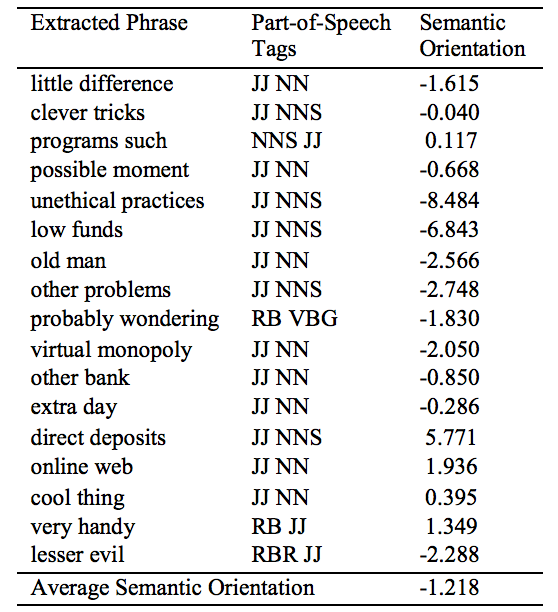
\includegraphics[width=0.65\textwidth]{turney06}
\end{center}
\end{frame} 


\begin{frame} \frametitle{Supervised Learning} %% 52

\fcolorbox{red}{white}{\parbox{0.9 \textwidth}{
 (Pang et al, 2002): ``Thumbs up?: sentiment classification using machine 
learning techniques.'' \\ \url{http://www.cs.cornell.edu/home/llee/papers/sentiment.pdf}
}}

\vfill

\begin{block}{}
Our aim in this work was to examine whether it sufficces to treat
sentiment classification simply as a special case of topic-based 
categorization (with the two ``topics'' being positive sentiment and
negative sentiment), or whether special sentiment-categorization 
methods need to be developed.
\end{block}

%% Directly apply supervised learning techniques to classify reviews into
%% positive and negative. \\
%% Like a text classification problem

\end{frame} 


\begin{frame} \frametitle{Supervised Learning} %% 52b


\begin{block}{ Classification techniques tried:}
\begin{enumerate}
\item Naive Bayes 
\item Maximum entropy 
\item Support vector machines
\end{enumerate}
\end{block}


\begin{block}{Features:} 

\begin{itemize}
\item negation tag, 
\item unigram (single words), 
\item bigram, 
\item POS tag, 
\item position.
\end{itemize}

\end{block}

\end{frame}


\begin{frame} \frametitle{Supervised Learning: Training and Test Data}


Movie reviews with star ratings
\begin{itemize}
\item 4-5 stars as positive 
\item 1-2 stars as negative
\end{itemize}

\vfill
Neutral is ignored. 

\vfill
SVM gives the best classification accuracy
\begin{itemize} 
\item 83\% 
\item Features: unigrams (bag of individual words)
\end{itemize}

\end{frame} 


\begin{frame} \frametitle{Supervised Learning: Outcome}

Accuracies achieved on the sentiment classification
problem smaller than standard topic-based 
categorization 
\begin{itemize}
\item Unigram presence information turned out to be the most
effective feature; 
\end{itemize}

\end{frame}


\begin{frame} \frametitle{The Need for Discourse Analysis}

(Pang et al. 2002): A common phenomenon was a kind of
\textbf{\em thwarted expectations} narrative, where the author sets up a
deliberate contrast to earlier discussion.


\begin{block}{}
  \small{ ``This film should be brilliant. It sounds like a great
    plot, the actors are first grade, and the supporting cast is good
    as well, and Stallone is attempting to deliver a good performance.
    \textbf{However, it can't hold up.}'' }

\end{block}

\vfill

\begin{block}{}
  \small{ ``I hate the Spice Girls.  ...[3 things the author hates
    about them]... Why I saw this movie is a really, really, really
    long story, but I did, and one would think I'd despise every
    minute of it. But... Okay, I'm really ashamed of it, but I enjoyed
    it. I mean, I admit it's a really awful movie ...the ninth floor
    of hell...The plot is such a mess that it's terrible.  \textbf{But I loved
    it.}''}
\end{block}

\end{frame}



\begin{frame} \frametitle{Features for Supervised Learning}


%% The problem has been studied by numerous researchers subsequently

Probably the most extensive studied problem
%% Including domain adaption and cross-lingual, etc.

\vfill 
\textbf{Key: feature engineering.} A large set of features have been tried. 

\begin{description}
\item [Term n-grams, frequency weighting schemes:] TF-IDF
  weighting scheme for unigrams (and bigrams) is common and quite effective
\item [Part of speech (POS) tags:] find adjectives. 
\item [Opinion words and phrases:] `` cost someone ar arm and a leg''
\item [Negations:] beware of ``not only...but also''
\item [Syntactic dependency:] features generated from parsing or
  dependency trees.
\end{description}

\end{frame} 


%%% advanced stuff -- SKIP

\begin{comment}

\begin{frame} \frametitle{Review Classification by Scoring Features }



\fcolorbox{red}{white}{\parbox{0.9 \textwidth}{
 (Dave, Lawrence and Pennock, WWW-03): ``Mining the peanut gallery:
opinion extraction and semantic classification of product reviews'' \\
\url{http://dl.acm.org/citation.cfm?id=775226} 
}}

\vfill

It first selects a set of features $F = f_1, f_2,...$ \\
Note: machine learning features, not product features. 

Score the features ($C$ and $C'$ are classes):

\begin{equation*}
score(f_i) = \frac{P(f_i | C) - P(f_i | C')}{P(f_i|C) +P(F_i|C')}
\end{equation*}

Classification of a  review $d_j$ (using sign): 

\begin{equation*}
class (d_j) = 
\begin{cases} 
C & \sum_i score(f_i) > 0\\
C' & \sum_i score(f_i) < 0
\end{cases}
\end{equation*}

Accuracy of 84 - 88\%. 

\end{frame}


\begin{frame} \frametitle{A large number of related papers} %%55

Bickerstaffe and Zukerman (2010) used a hierarchical multi-classifier considering inter-class similarity Burfoot, Bird and Baldwin (2011) sentiment-classified congressional floor debates Cui et al. (2006) evaluated some sentiment classification algorithms Das and Chen (2001) extracted market sentiment from stock message boards Dasgupta and Ng (2009) used semi-supervised learning Dave, Lawrence \& Pennock (2003) designed a custom function for classification Gamon (2004) classified customer feedback data
\end{frame} 

\begin{frame} \frametitle{A large number of related papers} %%56

Goldberg and Zhu (2006) used semi-supervised learning. Kim, Li and Lee (2009) and Paltoglou and Thelwall (2010) studied different IR term weighting schemes Li, Lee, et al (2010) made use of different polarity shifting. Li, Huang, Zhou and Lee (2010) used personal (I, we) and impersonal (they, it, this product) sentences to help Maas et al (2011) used word vectors which are latent aspects of the words. Mullen and Collier (2004) used PMI, syntactic relations and other attributes with SVM. Nakagawa, Inui and Kurohashi (2010) used dependency relations and CRF.
\end{frame} 

\begin{frame} \frametitle{A large number of related papers} %%57

Ng, Dasgupta and Arifin (2006) identified reviews and classified sentiments of reviews Pang and Lee (2004) used minimum cuts Qiu, Zhang, Hu and Zhao (2009) proposed a lexiconbased and self-supervision approach Tong (2001) used a set of domain specific phrases Yessenalina, Choi and Cardie (2010) automatically generated annotator rationales to help classification Yessenalina, Yue and Cardie (2010) found subjective sentences and then used them for model building Zhou, Chen and Wang (2010) used semi-supervised and active learning
\end{frame} 


\begin{frame} \frametitle{Review rating prediction}


Apart from classification of positive or negative sentiments, research
has also been done to predict the rating scores (e.g., 1­5 stars) of
reviews 

(Pang and Lee, 2005; Liu and Seneff 2009; Qu, Ifrim and Weikum
2010; Long, Zhang and Zhu, 2010). 

Training and testing are reviews with star ratings.


Formulation: The problem is formulated as regression since the rating scores are ordinal. Again, feature engineering and model building.
\end{frame} 

\begin{frame} \frametitle{Domain adaptation (transfer learning)}


Sentiment classification is sensitive to the domain of the training data.


A classifier trained using reviews from one domain often performs poorly in another domain.

words and even language constructs used in different domains for expressing opinions can be quite different. same word in one domain may mean positive but negative in another, e.g., ``this vacuum cleaner really sucks.''


Existing research has used labeled data from one domain and unlabeled
data from the target domain and general opinion words for learning

(Aue and Gamon 2005; Blitzer et al 2007; Yang et al 2006; Pan et al 2010; Wu, Tan and Cheng 2009; Bollegala, Wei and Carroll 2011; He, Lin and Alani 2011).

\end{frame} 

\begin{frame} \frametitle{Cross-lingual sentiment classification}


Useful in the following scenarios:


E.g., there are many English sentiment corpora, but for other languages (e.g. Chinese), the annotated sentiment corpora may be limited. Utilizing English corpora for Chinese sentiment classification can relieve the labeling burden.


Main approach: use available language corpora to train
sentiment classifiers for the target language data. Machine translation is typically employed

(Banea et al 2008; Wan 2009; Wei and Pal 2010; Kim et al. 2010; Guo et al 2010; Mihalcea \& Wiebe 2010; Boyd-Graber and Resnik 2010; Banea et al 2010; Duh, Fujino \& Nagata 2011; Lu et al 2011)

\end{frame} 

\end{comment}



\section{Sentence subjectivity \& sentiment classification} 


\begin{frame} \frametitle{Sentence-level Sentiment Analysis} %% BL62

\begin{itemize}
\item Document-level sentiment classification is too coarse for most applications. 
\item Much of the work on sentence level sentiment analysis focuses on identifying \textbf{subjective sentences} in news articles.
  \begin{itemize}\item Subjectivity Classification: objective and subjective. \end{itemize}
\item All techniques use some forms of machine learning, e.g., using a
  na\"ive Bayesian classifier with a set of data features/attributes
  extracted from training sentences % (Wiebe et al. ACL-99).
\end{itemize}
\end{frame}


\begin{frame} \frametitle{Sentence-level Sentiment Analysis} %% BL63


\begin{block}{Usually performed in two steps:}
\begin{enumerate}
\item Subjectivity classification \\
To identify subjective sentences 
\item Sentiment classification of subjective sentences \\
Into two classes, positive and negative
\end{enumerate}
\end{block}

\begin{block}{Bear in mind}
\begin{itemize}
\item Many objective sentences can imply sentiments 
\item Many subjective sentences do not express positive or negative sentiments/opinions \\
E.g., ``I believe he went home yesterday.''
\end{itemize}
\end{block}

\end{frame}



\begin{frame} \frametitle{Sentence-level Sentiment Analysis as an Intermediate Step} %% BL64


We do not use the quintuple $(e, a, so, h, t)$ to define the problem
here because sentence classification is an intermediate step.

\vfill

Knowing that some sentences have positive or negative opinions is not
sufficient, but helps: 
\begin{itemize}
\item filter out sentences with no opinions (mostly) 
\item determine (to some extent) if sentiments about entities and
  their aspects are positive or negative. 
\end{itemize}
\end{frame}


\begin{frame} \frametitle{Sentence-level Sentiment Analysis} %% BL65

\begin{block}{Assumption: }
Each sentence is written by a single person and expresses
a single positive or negative opinion/sentiment. 
\end{block}

\begin{itemize}
\item True for simple
sentences, e.g., \\
``I like this car''
\item Not true for compound and {\em complex} sentences, e.g., \\
``I like the picture quality but battery life sucks.'' \\
``Apple is doing very well in this lousy economy.''
\end{itemize}

\end{frame}


%%% advanced sentence-based classification, skip %%%

\begin{comment}

\begin{frame} \frametitle{Subjectivity Classification Using learnt
    patterns} %% BL66

 (Rilloff  and Wiebe, EMNLP-03) - A bootstrapping approach.

\begin{enumerate}
\item A high precision classifier is first used to automatically identify some subjective and objective sentences.

\begin{itemize}
    \item Two high precision (but low recall) classifiers are used,
      based on \textbf{manually collected lexical items, single words
        and n-grams}, which are good subjective clues.
      \begin{itemize} 
          \item a high precision subjective classifier 
          \item a high precision objective classifier 
       \end{itemize}
    \end{itemize}
\item A set of patterns are then learned from these identified subjective and objective sentences. \\
Syntactic templates are provided to restrict the kinds of patterns to be discovered, e.g., $<$subj$>$ passive-verb.

\item The learned patterns are then used to extract more subject and
  objective sentences\\
 (the process can be repeated). 
\end{enumerate}

\end{frame}


\begin{frame} \frametitle{Example Syntactic Templates}


\begin{tabular}{l l}
$<$subj$>$ passive-verb & $<$subj$>$  was satisfied \\
$<$subj$>$ active-verb & $<$subj$>$ complained \\
active-verb $<$dobj$>$ & endorsed $<$dobj$>$ \\
noun aux $<$dobj$>$  & fact is $<$dobj$>$ \\
passive-verb prep $<$np$>$ & was worried about $<$np$>$ \\

\end{tabular}
\end{frame}



\begin{frame} \frametitle{Subjectivity and Polarity (Orientation) } %% BL67


(Yu and Hazivassiloglou, EMNLP-03)

\begin{itemize}

\item For subjective or opinion sentence identification, three
  classification methods are benchmarked:
  \begin{itemize}
    \item Sentence similarity.
    \item Na\"ive Bayesian classification.
    \item Multiple na\"ive Bayesian (NB) classifiers. 
  \end{itemize}

\item For opinion orientation (positive, negative or neutral) (also
  called polarity) classification, it uses a similar method to
  (Turney, ACL-02), but 
  \begin{itemize}
    \item with more seed words (rather than two) and based on log-likelihood ratio (LLR). 
    \item For classification of each word, it takes the average of LLR
      scores of words in the sentence and use cutoffs to decide
      positive, negative or neutral
  \end{itemize}

\end{itemize}

\end{frame}

\end{comment}

%%% end of - advanced sentence-based classification %%%



% motivate Aspect-based here

\begin{frame} \frametitle{Let us go further?} %% BL73

\begin{itemize}
\item Sentiment classification at both document and sentence (or clause) levels are useful, but 
They do not find what the opinion holder liked and disliked.
  \begin{itemize}
    \item A negative sentiment on an entity does not mean that the opinion holder dislikes everything about the entity.
    \item A positive sentiment on an entity does not mean that the opinion holder likes everything about the entity.
  \end{itemize}
\end{itemize}

\colorbox{yellow}{\parbox{0.9 \textwidth} {\textbf{We need to go to the entity and aspect level.}}}

\end{frame}


\begin{frame} \frametitle{Sentiment Lexicon}

\colorbox{yellow}{\parbox{0.9 \textwidth} {A {\bf Sentiment Lexicon}
    is the key resource for sentiment analysis. How to generate one?}}

\vfill
Resources:
\begin{tabular}{l l}
SentiLex-PT & \url{http://dmir.inesc-id.pt/project/SentiLex-PT_02_in_English}\\
SentiWordNet & \url{ http://sentiwordnet.isti.cnr.it/} \\
Bing Liu's Lexicon & \url{http://www.cs.uic.edu/~liub/FBS/opinion-lexicon-English.rar}

\end{tabular}
\end{frame}

%% first lecture ends here %%%


\section{Opinion lexicon generation}


\begin{frame} \frametitle{Opinion (or sentiment) Lexicon} %% BL128


Opinion lexicon: lists of words and expressions used to express people's subjective feelings and sentiments/opinions.
\begin{itemize}
 \item Not just individual words, but also phrases and idioms, e.g., ``cost an arm and a leg''
\end{itemize}

\vfill
Instrumental for opinion mining. 

\vfill
There seems to be an endless variety of sentiment bearing expressions.
\begin{description} 
\item [Bing-Liu's Lexicon (EN):] more than 6,700 individual words. \\
There are also a large number of phrases.
\item [SentiLex PT 02:] more than 7000 entries. \\
Many expressions present as well
\end{description}


\end{frame}

% entradas SentiLex
% http://dmir.inesc-id.pt/project/SentiLex-PT_02_in_English


\begin{frame} \frametitle{Sentiment Lexicon} %% 129


Opinion words or phrases (also called polar words, opinion bearing words, etc). E.g.,

\begin{description}
\item [Positive:] beautiful, wonderful, good, amazing, 
\item [Negative:] bad, poor, terrible, {\em cost an arm and a leg.}
\end{description}

\vfill

Some opinion words are context independent (e.g., good).

\vfill
Some are context dependent (e.g., long).

\vfill

Some are domain dependent (e.g. scary)

\end{frame}


\begin{frame} \frametitle{Compiling a Sentiment Lexicon} %% 129

Three main ways to compile such lists:
\begin{description}  
\item [Manual approach: ] not a bad idea, if an one-time effort 
\item [Corpus-based approach ]
\item  [Dictionary-based approach]

\end{description}

\end{frame}



\begin{frame} \frametitle{Corpus-based approaches} %% 130 class + 131 class

% (Hazivassiloglou and McKeown, ACL-97; Turney, ACL-02; Yu and Hazivassiloglou, EMNLP-03; Kanayama and Nasukawa, EMNLP-06; Ding and Liu SIGIR-07)
%(Turney, ACL-02) and (Yu and Hazivassiloglou, EMNLP-03) are similar. 
%(Turney, ACL-02) and (Yu and Hazivassiloglou, EMNLP-03) are similar. 
%(Yu and Hazivassiloglou, EMNLP-03) is different from (Turney, ACL-02)
%use more seed words (rather than two) and use log-likelihood ratio (rather than PMI). 

Rely on syntactic or co-occurrence patterns in large corpora:
\begin{itemize}
\item Can find domain (not context!) dependent orientations (positive,
  negative, or neutral). 
\item Can asssign opinion orientations (polarities) to words/phrases.
\end{itemize}

\vfill
 % (Hazivassiloglou and McKeown, ACL-97; Kanayama and Nasukawa,
 % EMNLP-06; Ding and Liu, 2007). E.g.,
% (Hazivassiloglou and McKeown, ACL-97): 
Use constraints (or conventions) on connectives to identify  opinion words
\begin{itemize}
\item Conjunction: conjoined adjectives usually have the same
  orientation (Hazivassiloglou and McKeown, ACL-97):\\
E.g., ``This car is beautiful and spacious.'' (conjunction)
\item AND, OR, BUT, EITHER-OR, and NEITHER-NOR: similar constraints.
\item Learning using 
\begin{description}
    \item [log-linear model:] determine if two conjoined adjectives are of the same or different orientations. 
    \item [Clustering:] produce two sets of words: positive and negative
    %\item Corpus: 21 million word 1987 Wall Street Journal corpus. 
\end{description}
\end{itemize}
\end{frame}


% it would be instructive to include here mores slides detailing
% (Hazivassiloglou and McKeown, ACL-97;)
% next year

\begin{comment}

\begin{frame} \frametitle{Corpus-based Approaches (contd)} %% class

(Kanayama and Nasukawa, EMNLP-06) takes a similar approach to
(Hazivassiloglou and McKeown, ACL-97) but for Japanese words:
\begin{itemize}
\item Instead of using learning, it uses two criteria to determine whether to add a word to positive or negative lexicon. 
\item Have an initial seed lexicon of positive and negative words.
\end{itemize}

\end{frame}


\begin{frame} \frametitle{Corpus-based Approaches (contd)} %% class
 
(Ding and Liu, 2007) also exploit constraints on connectives, but
with a twist:
\begin{itemize}
\item It uses them to assign opinion orientations to product aspects (more on this later). 
\begin{itemize}
  \item One word may indicate different opinions in the same domain. \\
``The battery life is long'' (+) and ``It takes a long time to focus'' (-).
  \item Finding domain opinion words is insufficient. 
\end{itemize}
\item It can be used without a large corpus.
\end{itemize}

\end{frame}


\begin{frame} \frametitle{Find Domain Opinion Words} %% 132 

A similar approach was also taken in (Kanayama and Nasukawa, 2006) but for Japanese words:


Instead of only based on intra-sentence sentiment consistency, the new method also looks at the previous and next sentence, i.e., inter-sentence sentiment consistency. Have an initial seed lexicon of positive and negative words.

\end{frame}

\begin{frame} \frametitle{Context-dependent Opinion} %%133 


Find domain opinion words is insufficient. A word may indicate different opinions in same domain.


``The battery life is long'' (+) and ``It takes a long time to focus'' (-).


Ding, Liu and Yu (2008) and Ganapathibhotla and Liu (2008) exploited sentiment consistency (both inter and intra sentence) based on contexts
  

It finds context dependent opinions. Context: (adjective, aspect), e.g., (long, battery\_life) It assigns an opinion orientation to the pair.


\end{frame}

\end{comment}


\begin{frame} \frametitle{The Double Propagation Method} %% 134 class


\fcolorbox{red}{white}{\parbox{0.9 \textwidth}{
(Qiu et al., 2010): ``Opinion Word Expansion and Target Extraction through
Double Propagation.'' \\
 Computational Linguistics, Vol. 37, No. 1: 9.27, 2010.
}}

A double propagation method:
\begin{itemize}
\item Explores dependency relations of opinions and aspects to
    extract opinion words.
  \begin{itemize}
    \item Opinion words modify entity aspects/features, e.g., \\
        ``This camera has \textcolor{red}{long} \textcolor{blue}{battery life}''
  \end{itemize}
   
\item The algorithm essentially bootstraps using a set of seed opinion
  words with the help of some dependency relations.
  \begin{itemize}
    \item Knowing an aspect, one can find the opinion word that
modifies it: ``The \textcolor{blue}{rooms} are
\textcolor{red}{spacious}''
    \item Knowing some opinion words, one can find more opinion words: ``The rooms are \textcolor{blue}{spacious} and \textcolor{red}{beautiful}''
  \end{itemize}
\end{itemize}

\end{frame}



\begin{comment}

from: Qiu, G., B. Liu, J. Bu, and C. Chen. Opinion Word Expansion and Target Extraction through
Double Propagation. Computational Linguistics, Vol. 37, No. 1: 9.27, 2010.

In this article, we propose a novel propagation based method to solve
the opinion lexicon expansion and target extraction problems
simultaneously. Our approach differs from existing approaches in that
it requires no additional resources except an initial seed opinion
lexicon, which is readily available. Thus, it can be seen as a
semi-supervised method due to the use of the seeds. It is based on the
observation that there are natural relations between opinion words and
targets due to the fact that opinion words are used to modify
targets. Furthermore, we find that opinion words and targets themselves
have relations in opinionated expressions too. These relations can be
identified via a dependency parser based on the dependency grammar
(Tesniere 1959), and then exploited to perform the extraction tasks.

The basic idea of our approach is to extract opinion words (or
targets) iteratively using known and extracted (in previous
iterations) opinion words and targets through the identification of
syntactic relations. The identification of the relations is the key to
the extractions. As our approach propagates information back and forth
between opinion words and targets, we call it double
propagation. 

Opinion word sentiment or polarity assignment (positive,
negative, or neutral) and noisy target pruning methods are also
designed to refine the initially extracted results. 

In evaluation, we
compare our approach with several state-of-the-art existing approaches
in opinion lexicon expansion (or opinion word extraction) and target
(or feature/topic) extraction. The results show that our approach
outperforms these existing approaches significantly



\begin{frame} \frametitle{Rules from Dependency Grammar} %% Class

\begin{center}
     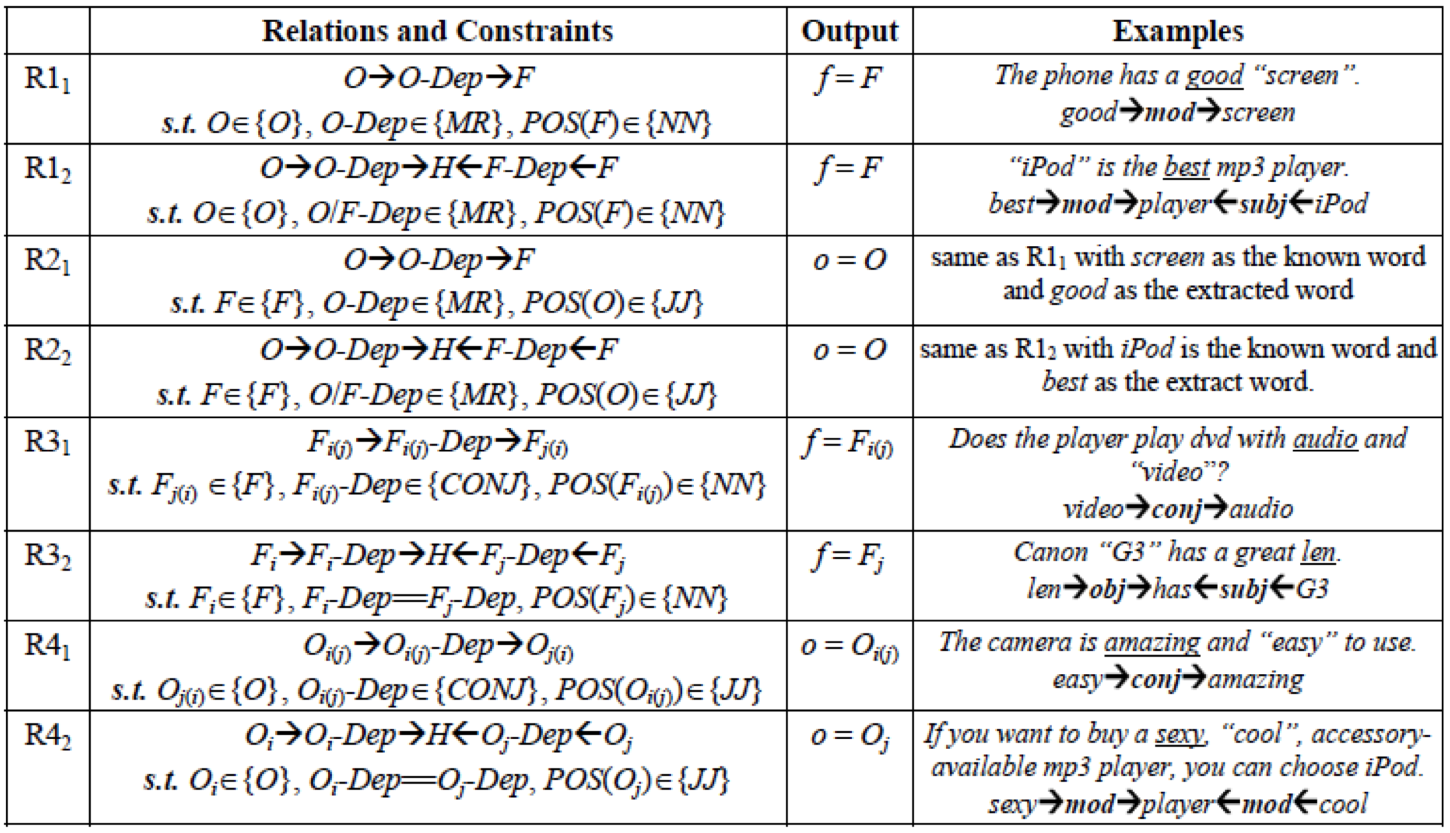
\includegraphics[width=0.95\textwidth]{rules-dependency-grammar}
\end{center}

\tiny{Column (1) is the rule ID, (2) is observed dependency and the constraint that
  it must satisfy (after s.t.), (3) is the output, and (4)
  is an example. In each example, the underlined word is the known
  word and the word with double quotes is the extracted word. We also
  show the corresponding instantiated dependency in the parentheses.
}
\end{frame}




\begin{frame} \frametitle{Opinions Implied by Objective Terms} %% 135

% (Zhang and Liu, 2011a)

\vfill
Most opinion words are adjectives and adverbs, e.g., good, bad, etc

There are also many subjective and opinion verbs and nouns, e.g., hate
(VB), love (VB), crap (NN). E.g., ``After sleeping on the mattress for
one month, a valley/body impression has formed in the middle.'' 

But objective nouns can imply opinions too.

How to discover such nouns in a domain or context?

\end{frame}

\begin{frame} \frametitle{The Technique} %% 136


Sentiment analysis to determine whether the context is +ve or ­ve. \\
``I saw a valley in two days, which is terrible.''  This is a negative context.

Statistical test to find +ve and ­ve candidates.

Pruning to move those unlikely ones though sentiment homogeneity.

\end{frame}

\begin{frame} \frametitle{Pruning} %% 137

For an aspect with an implied opinion, it has a fixed opinion, either +ve or ­ve, but not both. We find two direct modification relations using a dependency parser.

Type 1: O  O-Dep  A \\
e.g. ``This TV has good picture quality.'' e.g. ``The springs of the mattress are bad.''


Type 2: O  O-Dep  H  A-Dep  A \\
If an aspect has mixed opinions based on the two dependency relations, prune it.


\end{frame}

\begin{frame} \frametitle{Opinions implied by resource usage} %% BL 138

(Zhang and Liu, 2011b)

\vfill
Resource usage descriptions may also imply opinions (as mentioned in
rules of opinions) \\
E.g., ``This washer uses a lot of water.'' 

\vfill 
Two key roles played by resources usage:
\begin{enumerate}
\item An important aspect of an entity, e.g., water usage. 
\item Imply a positive or negative opinion
\end{enumerate}

\vfill
Resource usages that imply opinions can often be described by a triple.
\begin{equation*}
(verb, quantifier, noun\_term), 
\end{equation*}

Verb: uses, quantifier: ``a lot of'', noun\_term: water


\end{frame}

\begin{frame} \frametitle{The Proposed Technique} % 139


The proposed method is graph-based.

Stage 1: Identifying Some Global Resource Verbs

Identify and score common resource usage verbs used in almost any domain, e.g., ``use'' and ``consume''

Stage 2: Discovering Resource Terms in each Domain Corpus


Use a graph-based method considering occurrence probabilities. With resource verbs identified from stage 1 as the seeds. Score domain specific resource usage verbs and resource terms.

\end{frame}

\end{comment}

%%%%%% Dictionary-based approaches %%%%%%%%%%

\begin{frame} \frametitle{Dictionary-based Approaches} %% BL 140 class

Typically use WordNet's synsets and hierarchies to acquire opinion words

\begin{itemize}
\item Start with a small seed set of opinion words. 
\item Bootstrap the set to search for synonyms and antonyms in WordNet
  iteratively % (Hu and Liu, 2004; Kim and Hovy, 2004; Kamps et al 2004).
\item Use the set to search for synonyms and antonyms in WordNet % (Hu and Liu, KDD-04; Kim and Hovy, COLING-04).
\end{itemize}
 
\vfill
Manual inspection may be used afterward.
% Use additional information (e.g., glosses) from WordNet (Andreevskaia and Bergler, EACL-06) and learning (Esuti and Sebastiani, CIKM-05).
% (Dragut et al 2010) uses a set of rules to infer orientations.

\vfill
Weakness of the approach: Does not find context dependent opinion words, e.g., small, long, fast. 

\end{frame}


\begin{comment}

\begin{frame} \frametitle{Semi-supervised Learning} %% BL 141

(Esuti and Sebastiani, 2005)


\vfill
Use supervised learning 

Given two seed sets: positive set P, negative set N The two seed sets are then expanded using synonym and antonymy relations in an online dictionary to generate the expanded sets P' and N'.

P' and N' form the training sets. Using all the glosses in a dictionary for each term in P'  N' and converting them to a vector

Build a binary classifier

Tried various learners.

\end{frame}

\begin{frame} \frametitle{Multiple Runs of Bootstrapping} %% BL 142

% (Andreevskaia and Bergler, 2006)

Basic bootstrapping with given seeds sets (adjectives)

\begin{itemize}
\item First pass: seed sets are expanded using synonym, antonymy, and
hyponyms relations in WordNet. 

\item Second pass: it goes through all WordNet glosses and identifies the
entries that contain in their definitions the sentiment-bearing words
from the extended seed set and adds these head words to the
corresponding category (+ve, -ve, neutral) 

\item Third pass: clean up using a POS tagger to make sure the words are adjectives and remove contradictions.
\end{itemize}

\end{frame}

\begin{frame} \frametitle{Multiple runs of bootstrapping (contd)} %% BL 143

\begin{itemize}
\item Each word is then assigned a fuzzy score reflecting the degree of
certainty that the word is opinionated (+ve/-ve). 

\item The method performs multiple runs of bootstrapping using non-overlapping seed sets.
\begin{itemize}
\item A net overlapping score for each word is computed based on how many
times the word is discovered in the runs as +ve (or ­ve) 
\item The score is normalized based on the fuzzy membership.
\end{itemize}
\end{itemize}

\end{frame}

\end{comment}


\begin{frame} \frametitle{SentiLex-PT}


\fcolorbox{red}{white}{\parbox{0.9 \textwidth}{
(Silva et al., 2012): ``Building a
Sentiment Lexicon for Social Judgement Mining'' \\
 International Conference on Computational Processing of
Portuguese (PROPOR), 2012}}

\vfill SentiLex web page: \\
\url{http://dmir.inesc-id.pt/project/SentiLex-PT_02_in_English}

\end{frame}

\begin{frame} \frametitle{SentiLex-PT}

\begin{itemize}
\item Combined 4 dictionaries of synonyms, among which Papel \url{http://www.linguateca.pt/PAPEL/papel.html}

\item Used a pattern approach to identify human adjectives

\item Classification seeds: Manually classified polarity for a set of lemmas

\item Generated a network of lemmas, based on synonimity relationships

\item Applied a propagation procedure, based on distance, computed with
Djiskstra's shortest-path algorithm, to special nodes ``1'', ``0'',
``-1'' connected to pos/neu/neg seeds.
\end{itemize}

\end{frame}



\begin{frame} \frametitle{Shortcomings of the Dictionary-based
    Approach} % extra -- pcc 

Unable to find opinion words with domain specific orientations:
\begin{center}
\begin{tabular}{ll}
\textbf{nervous} car  & \textbf{nervous} person \\
long battery life & long explanation \\
small digital camera & small house \\
Clooney is a really \textbf{good} actor  & Obama is a really \textbf{good} actor
\end{tabular}

\end{center}
\end{frame}

\begin{frame} \frametitle{Which Approach is Best?} %% 144

The corpus and dictionary-based approaches complement each other.
\begin{itemize}
\item The dictionary does not usually give domain or context dependent meaning\\
A corpus is needed for that

\item It is hard to find a corpus with a very large set of opinion words \\
A dictionary is good for that
\end{itemize}

\colorbox{yellow}{\parbox{0.9 \textwidth} {
In practice, the corpus, dictionary and manual approaches are all needed.
}}

\end{frame}


\begin{comment}

\begin{frame} \frametitle{Some other related papers} %% 145


Choi and Cardie (2009) adapting a lexicon to domain specific need
using integer linear programming 

Du and Tan (2009) and Du, Tan, Cheng and Yun (2010) clustered
sentiment words 

Hassan and Radev (2010) built a word graph based on synonyms and then
used a number of random walks to hit known seed words 

Hassan et al. (2011) found sentiment orientations of foreign words. It
first created a multilingual word network and then did random walk
similar to the above paper. 

Jijkoun, Rijke and Weerkamp (2010) used target and sentiment word relationship. Similar to that in (Qiu et al 2009).

\end{frame}

\begin{frame} \frametitle{Some other related papers} %% 146


Kaji and Kitsuregawa (2006, 2007) and Velikovich et al (2010) used
text on the web to generate lexicons. 

Lu et al (2011) dealt with the same problem as (Ding et al 2008) but
used various constraints in optimization. 

Mohammad, Dunne, and Dorr, (2009) used seeds and thesaurus. 

Rao and Ravichandran (2009) used WordNet and OpenOffice thesaurus and
semi-supervised learning 

Wu and Wen (2010) found context adjectives like large and small by
mining the web using lexico-syntactic patterns. \\
They solved the same problem as (Ding et al 2008)

\end{frame}
\end{comment}



\section{Aspect-based sentiment analysis \& opinion summarization}


\begin{frame} \frametitle{Aspect-based Sentiment Analysis} %% BL 73

\fcolorbox{red}{white}{\parbox{0.9 \textwidth}{\textbf{We have to get to People's Sentiment:} 
Sentiment classification at both the document and sentence (or clause)
levels is useful, but that does not tell what people liked and disliked. 
}}

\vfill
Have to identify the targets of opinions, i.e., \textbf{\textcolor{blue}{entities} and their \textcolor{blue}{aspects}} 

\vfill
Without knowing targets, opinions are of limited use. We thus need the full opinion definition.


%We need to go to the entity and aspect level.
%Aspect-based opinion mining and summarization (Hu and Liu 2004). 

\end{frame}

\begin{frame} \frametitle{Opinion is a Quintuple} %% 74


\begin{equation*}
(e_i, a_{jk}, so_{ijkl}, h_k, t_l)     
\end{equation*}

\begin{description}
\item [$e_j$]  a target entity
\item [$a_{jk}$] an aspect of $e_j$
\item [$so_{ijkl}$]  is the sentiment value of the opinion of the opinion holder $h_i$ on feature $a_{jk}$ of entity $e_j$ at time $t_l$
\item [$h_i$] is an opinion holder
\item [$t_l$] is the time when the opinion is expressed. 
\end{description}



\end{frame}

\begin{frame} \frametitle{Reviews and Blogs} %% BL75
 
\begin{itemize}
\item  Much of the research is based on online reviews 
\item For reviews, aspect-based sentiment analysis is easier because
  the entity (i.e., product name) is usually known \\
Reviewers simply express positive and negative opinions on different aspects of the entity.

\item For blogs, forum discussions, etc., it is harder: \\
both entity and aspects of entity are unknown, \\
there may also be  many comparisons, and \\
there is also a lot of irrelevant information.

\end{itemize}

\end{frame}

\begin{frame} \frametitle{Find Entities (entity set expansion)} %% BL76

\begin{itemize}
\item Although similar, it is somewhat different from the traditional named entity recognition (NER).
\item E.g., one wants to study opinions on phones \\
given Motorola and Nokia, find all phone brands and models in a corpus, e.g., Samsung, Moto
\end{itemize}

\begin{block}{Formulation:} 
Given a set Q of seed entities of class C, and a set D of candidate entities, we wish to determine which of the entities in D belong to C.
\end{block}

It needs a binary decision for each entity
in D (belonging to C or not) \\
A classification problem  often solved as a ranking problem

\end{frame}


\begin{comment}
\begin{frame} \frametitle{Some Methods}  %% 77

 %(Li, Zhang et al 2010, Zhang and Liu 2011)

\begin{description}
\item [Distributional similarity:] This is the traditional method used in NLP. It compares the surrounding text of candidates using cosine or PMI.\\
It performs poorly.
\item [PU learning:] learning from positive and unlabeled examples.\\
S-EM algorithm (Liu et al. 2002)
\item [Bayesian Sets:] Extended the method given in (Ghahramani and Heller, 2006).
\end{description}
\end{frame}

\end{comment}

\begin{frame} \frametitle{Aspect Extraction} %% BL78

\begin{block}{Goal:}
Given an opinion corpus, extract all aspects 
\end{block}


\vfill

\begin{itemize}

\item A frequency-based approach (Hu and Liu, 2004): nouns (NN) that
  are frequently talked about are likely to be true aspects (called
  frequent aspects) . 

\item Why the frequency based approach? \\
Different reviewers tell different stories (irrelevant) \\
When product aspects/features are discussed, the words they use
converge. \\
They are the main aspects.

\item Sequential/association pattern mining finds frequent nouns and noun phrases.

\end{itemize}


\end{frame}

\begin{frame} \frametitle{An Example Review} %% BL79

\begin{block}{\textbf{GREAT Camera}, Jun 3, 2004 Reviewer: \textbf{jprice174} from Atlanta, Ga.}

\textcolor{green}{
I did a lot of research last year before I bought this camera... It
kinda hurt to leave behind my beloved nikon 35mm SLR, but I was going
to Italy, and I needed something smaller, and digital. 
}

The \textcolor{red}{pictures} coming out of this camera are amazing. The \textcolor{red}{'auto'} feature
takes great \textcolor{red}{pictures} most of the time. And with digital, you're not
wasting film. ...\\
....
\end{block}

\end{frame}

\begin{frame} \frametitle{Infrequent Aspect Extraction} %% BL80

Infrequent aspects: use opinion words to extract the aspects. 

\textbf{Key idea:} \textcolor{blue}{opinions have targets}, i.e., opinion words are used to modify aspects and entities.
 \begin{itemize}
\item ``The pictures are absolutely \textcolor{blue}{amazing}.'' 
\item ``This is an \textcolor{blue}{amazing} software.''
\end{itemize}

The modifying relation was approximated with the nearest noun to the
opinion word. 
\begin{itemize}
\item The idea was generalized to dependency in (Zhuang et al 2006) and
double propagation in (Qiu et al 2009;2011). \\
It has been used in many papers and practical systems
\end{itemize}

\end{frame}

\begin{comment}

\begin{frame} \frametitle{Using part-of relationship and the Web} %% 81

(Popescu and Etzioni, 2005)

Improved (Hu and Liu, 2004) by removing those frequent noun phrases that may not be aspects: better precision (a small drop in recall). It identifies part-of relationship

Each noun phrase is given a pointwise mutual information score between the phrase and part discriminators associated with the product class, e.g., a scanner class. E.g., ``of scanner'', ``scanner has'', etc, which are used to find parts of scanners by searching on the Web:

hits (a  d ) PMI (a, d ) = , hits (a )hits (d )



\end{frame}


\begin{frame} \frametitle{Extract aspects using DP}  %% 82
 
 (Qiu et al. 2009; 2011)

\vfill
A double propagation (DP) approach proposed 

Based on the definition earlier, an opinion should have a target, entity or aspect. Use dependency of opinions \& aspects to extract both aspects \& opinion words.
 

Knowing one helps find the other. E.g., ``The rooms are spacious''


It extracts both aspects and opinion words.  A domain independent method.

\end{frame}

\begin{frame} \frametitle{The DP method} %% 83


DP is a bootstrapping method
 

Input: a set of seed opinion words, no aspect seeds needed "This phone has good screen"


Based on dependency grammar (Tesniere 1959).

\end{frame}

\begin{frame} \frametitle{Rules from Dependency Grammar} %%  84

\end{frame}

\end{comment}

\begin{frame} \frametitle{Explicit and Implicit Aspects} %% 85

(Hu and Liu 2004)

\begin{itemize}
\item \textbf{Explicit aspects:} Aspects explicitly mentioned as nouns
  or noun phrases in a sentence 
\begin{itemize}
\item ``The \textcolor{blue}{picture quality} is of this phone is great.''
\end{itemize}

\item \textbf{Implicit aspects:} Aspects which are not explicitly
  mentioned in a sentence but are implied 
\begin{itemize}
\item ``This car is so \textcolor{blue}{expensive}.'' 
\item ``This phone will not easily \textcolor{blue}{fit in a pocket.}'' 
\item ``Included \textcolor{blue}{16MB} is stingy''
\end{itemize}

\end{itemize}

Not much work has been done on mining or mapping implicit aspects.


\end{frame}


\begin{frame} \frametitle{Mapping Implicit Aspects} %% 86


There are many types of implicit aspect expressions. 
\begin{itemize}
\item Adjectives and adverbs are perhaps the most common type.
\item Most adjectives modify or describe some specific attributes of
  entities \\ 
\begin{tabular}{lcl}
``expensive'' & $\Rightarrow$ & aspect ``price'' \\
``beautiful''  & $\Rightarrow$ & aspect ``appearance''  \\
``heavy''  &  $\Rightarrow$ & aspect ``weight''
\end{tabular}

\end{itemize}


\vfill
Although manual mapping is possible, in different contexts the meaning can be different.
\begin{itemize}
\item ``The computation is \textcolor{blue}{expensive}''.
\end{itemize}

\end{frame}


\begin{comment}

\begin{frame} \frametitle{A Mutual Reinforcement Method} %% 87

% (Su et al. 2009)

It proposed an unsupervised approach which exploits the mutual reinforcement relationship between aspects and opinion words.


Specifically, it uses the co-occurrence of aspect and opinion word pair in a sentence.


The algorithm iteratively clusters the set of aspects and the set of
opinion words separately, but before clustering each set, clustering
results of the other set is used to update the pairwise weight of the
set. The model is based on a bipartite graph.


\end{frame}

\end{comment}

\begin{comment}

\begin{frame} \frametitle{Other papers on aspect extraction} %% 88
We will discuss topic modeling based methods later.  

Carvalho et al (2011) annotated political debates with aspects and
others. 

Choi and Cardie (2010) used a CRF based approach. Jin and Ho (2009) proposed a HMM-based method Jakob and Gurevych (2010) used anaphora (or coreference) resolution to help find aspects that are mentioned in previous sentences but are referred to as pronouns in the next sentences.

E.g., ``I took a few pictures yesterday. They look great.'' There is almost no improvement with anaphora resolution, higher recall but lower precision.

\end{frame}

\begin{frame} \frametitle{Other papers on aspect extraction} %%89

Jakob and Gurevych (2010) used CRF to train on review sentences from
different domains for a more domain independent extraction. 

A set of domain independent features were used, e.g. tokens, POS tags,
dependency, word distance, and opinion sentences. Kobayashi et al
(2006) extracted subject-attribute-value Kobayashi et al (2007)
extracted aspect-evaluation and aspect-of relations using mined
patterns. 


Ku et al. (2006a, 2006b) performed the extraction from Chinese reviews and news.

\end{frame}

\begin{frame} \frametitle{Other papers on aspect extraction} %%90


Li et al (coling-2010) integrated Skip-CRF and Tree-CRF to extract
aspects and opinions.

It was able to exploit structure features 

Long, Zhang and Zhu (2010) extracted aspects (nouns) based on
frequency and the Web, and dependent words (adjectives).

These words are then used to select reviews which discuss an aspect
most.

Ma and Wan (2010) used centering
theory for extraction in news comments. It also exploited aspects in
the news title and contents. 

Meng and Wang (2009) extracted aspects from product specifications, which are usually structured data.
\end{frame}

\begin{frame} \frametitle{Other papers on aspect extraction} %% 91

Scaffidi et al (2007) extracted frequent nouns and noun phrases but
compare their frequency in a review corpus with their occurrence rates
in generic English to identify true aspects Somasundaran and Wiebe
(2009) also used syntactic dependency for aspect and opinion
extraction. 

Toprak, Jakob and Gurevych (2010) designed a comprehensive annotation
scheme for aspect-based opinion annotation.

Earlier annotations are partial and mainly for individual papers. 

Yi et al (2003) used language models to extract product features.

\end{frame}

\begin{frame} \frametitle{Other papers on aspect extraction} %92

Yu et al (2011) ranked aspects by considering their frequency and
contribution to the overall review rating 

Zhu et al (CIKM-2009) used a method for finding multiword terms, called cvalue, to find aspects.

The method also segments a sentence with multiple aspects.

\end{frame}


\end{comment}


\begin{frame} \frametitle{Identify Aspect Synonyms } %%93

(Carenini et al.  2005)

\vfill
Once aspect expressions are discovered, group them into aspect categories.\\
E.g., power usage and battery life are the same.

\vfill
Method based on some similarity metrics, but it needs a taxonomy of aspects.
\begin{itemize}
\item The system merges each discovered aspect to a aspect node in the
taxonomy.
\item Similarity metrics: string similarity, synonyms and other distances measured using WordNet.
\end{itemize}

\vfill
Many ideas in Web information integration are applicable

\end{frame}


\begin{comment}

\begin{frame} \frametitle{Multilevel Latent Categorization} %%94

(Guo et al 2009)


This method performs multilevel latent semantic analysis to group aspects expressions.


At the first level, all the words in aspect expressions are grouped into a set of concepts using LDA. The results are used to build latent topic structures for aspect expressions, e.g.,

touch screen: topic-1, topic-2

At the second level, aspect expressions are grouped by LDA again according to
 
their latent topic structures produced from level 1 and context snippets in reviews.



\end{frame}

\begin{frame} \frametitle{Group Aspect Synonyms} %% 95

 (Zhai et al. 2011a,  b)


A variety of information/similarities are used to cluster aspect expressions into aspect categories.
  

Lexical similarity based on WordNet Distributional information (surrounding words context) Syntactical constraints (sharing words, in the same sentence) Clustering: EM-based. Constrained topic modeling: Constrained-LDA




Two unsupervised learning methods were used:
 

By intervening Gibbs sampling.


\end{frame}

\begin{frame} \frametitle{The EM method} %% 96


WordNet similarity



EM-based probabilistic clustering

\end{frame}

\begin{frame} \frametitle{Aspect sentiment classification} %% 97


For each aspect, identify the sentiment or opinion expressed on it. Work based on sentences, but also consider,
 

A sentence can have multiple aspects with different opinions. E.g., The battery life and picture quality are great (+), but the view founder is small (-).



Almost all approaches make use of opinion words and phrases. But notice:




Some opinion words have context independent orientations, e.g., "good" and "bad" (almost) Some other words have context dependent orientations, e.g., "small" and "sucks" (+ve for vacuum cleaner)





\end{frame}

\begin{frame} \frametitle{Some Approaches} %%98


Supervised learning


Sentence level classification can be used, but ...

Need to consider target and thus to segment a sentence (e.g., Jiang et al. 2011)

Need parsing to deal with: 

Simple sentences, compound sentences,
comparative sentences, conditional sentences, questions; different
verb tenses, etc. 

Negation (not), contrary (but), comparisons, etc. 

A large opinion lexicon, context dependency, etc. Easy: ``Apple is doing well in this bad economy.''




Lexicon-based approach (Ding, Liu and Yu, 2008)


\end{frame}

\begin{frame} \frametitle{A Lexicon-based Method} %% BL99
  
 (Ding, Liu and Yu 2008)


Input: A set of opinion words and phrases. A pair (a, s), where a is
an aspect and s is a sentence that contains a. Output: whether the
opinion on a in s is +ve, -ve, or neutral. 

Two steps:  

Step 1: split the sentence if needed based on BUT words (but, except
that, etc). 

 Step 2: work on the segment sf containing a. Let the set of opinion words in sf be w1, .., wn. Sum up their orientations (1, -1, 0), and assign the orientation to (a, s) accordingly. wi .o n i =1 d (w , a) i where wi.o is the opinion orientation of wi. d(wi, a) is the distance from a to wi.





\end{frame}

\begin{frame} \frametitle{Sentiment shifters}  % (e.g., Polanyi and Zaenen 2004) %%100


Sentiment/opinion shifters (also called valence shifters are words and phrases that can shift or change opinion orientations. Negation words like not, never, cannot, etc., are the most common type. Many other words and phrases can also alter opinion orientations. E.g., modal auxiliary verbs (e.g., would, should, could, etc)


``The brake could be improved.''

\end{frame}

\begin{frame} \frametitle{Sentiment shifters (contd)} %% 101


Some presuppositional items also can change opinions, e.g., barely and hardly
 

``It hardly works.'' (comparing to ``it works'') It presupposes that
better was expected. ``This camera fails to impress me.'' ``What a great car, it did not start the first day.''


Words like fail, omit, neglect behave similarly,


Sarcasm changes orientation too

Jia, Yu and Meng (2009) designed some rules based on parsing to find the scope of negation.


\end{frame}

\begin{frame} \frametitle{Basic rules of opinions} %%102

 (Liu, 2010)

\vfill
Opinions/sentiments are governed by many rules, e.g.,


Opinion word or phrase, ex: "I love this car"
P N ::= ::= a positive opinion word or phrase an negative opinion word or phrase



Desirable or undesirable facts, ex: "After my wife and I slept on it for two weeks, I noticed a mountain in the middle of the mattress"
P N ::= ::= desirable fact undesirable fact


\end{frame}

\begin{frame} \frametitle{Basic rules of opinions} %% 103


High, low, increased and decreased quantity of a positive or negative potential item, ex: "The battery life is long."
PO ::= | NE ::= | NPI ::= PPI ::= no, low, less or decreased quantity of NPI large, larger, or increased quantity of PPI no, low, less, or decreased quantity of PPI large, larger, or increased quantity of NPI a negative potential item a positive potential item


\end{frame}

\begin{frame} \frametitle{Basic rules of opinions} %% 104


Decreased and increased quantity of an opinionated item, ex: "This drug reduced my pain significantly."
PO NE ::= | ::= | less or decreased N more or increased P less or decreased P more or increased N



Deviation from the desired value range: "This drug increased my blood pressure to 200."
PO NE ::= within the desired value range ::= above or below the desired value range





\end{frame}

\begin{frame} \frametitle{Basic rules of opinions} %% 105


Producing and consuming resources and wastes, ex: ``This washer uses a lot of water''
PO ::= | | | ::= | | | produce a large quantity of or more resource produce no, little or less waste consume no, little or less resource consume a large quantity of or more waste produce no, little or less resource produce some or more waste consume a large quantity of or more resource consume no, little or less waste


NE




\end{frame}

\begin{frame} \frametitle{Sentiment ontology tree} %% BL 106

 (Wei and Gulla,  2010)

Recall in the definition of opinions, we simplified the tree structure to two levels (entity \& aspects). This paper uses a full tree ontology to denote the relationships of aspects of a product.

\end{frame}

\begin{frame} \frametitle{Sentiment ontology tree (contd)} %% BL 107




The leaves of the tree are positive or negative sentiments. It then uses a hierarchical classification model to learn to assign an sentiment to each node, which is reflected as a child leaf node.


Hierarchical classifier is useful here because it considers parents when classifying children.



However, the ontology for each product has to be built manually.





\end{frame}

\begin{frame} \frametitle{Aspect-sentiment statistical models} %% 108


This direction of research is mainly based on topic models:
 

pLSA: Probabilistic Latent Semantic Analysis (Hofmann 1999) LDA: Latent Dirichlet allocation (Blei, Ng \& Jordan, 2003;
Griffiths \& Steyvers, 2003; 2004)


Topic models:
 
documents are mixtures of topics a topic is a probability distribution
over words.

 it specifies a simple probabilistic procedure by which documents can be generated.




A topic model is a document generative model





\end{frame}

\begin{frame} \frametitle{Aspect-sentiment model (Mei et al 2007)} %% BL 109
 

This model is based on pLSA (Hofmann, 1999). 

It builds a topic (aspect) model, a positive sentiment model, and a negative sentiment model. A training data is used to build the initial models.


Training data: topic queries and associated positive and negative sentences about the topics.


The learned models are then used as priors to build the final models on the target data. Solution: log likelihood and EM algorithm

\end{frame}

\begin{frame} \frametitle{Multi-Grain LDA to extract aspects} %% BL 110

(Titov and McDonald, 2008a, 2008b)


Unlike a diverse document set used for traditional topic modeling. All reviews for a product talk about the same topics/aspects. It makes applying PLSA or LDA in the traditional way problematic. Multi-Grain LDA (MG-LDA) models global topics and local topics (Titov and McDonald, 2008a).
 
Global topics are entities (based on reviews) Local topics are aspects (based on local context, sliding windows of review sentences)

MG-LDA was extended to MAS model to give aspect rating (Titov and McDonald, 2008b).

\end{frame}

\begin{frame} \frametitle{Aspect-rating of short text} %% BL 111

 (Lu et al    2009)

This work makes use of short phrases, head terms (wh) and their modifiers (wm), i.e.
 

(wm, wh) 

E.g., great shipping, excellent seller
 

Objective: (1) extract aspects and (2) compute their ratings in each
short comment. 

It uses pLSA to extract and group aspects It uses existing rating for the full post to help determine aspect ratings.


\end{frame}

\begin{frame} \frametitle{Aspect-rating regression} %% 112

% (Wang, Lu, and Zhai, 2010)


In this work, some seed aspects are given. Its first step finds more
aspect words using a heuristic bootstrapping method. 

Its regression model makes use of the review rating and assumes the overall review
rating is a linear combination of its aspect ratings. 

The problem is model as a Bayesian regression problem.


It is solved using log-likelihood and EM.

\end{frame}

\begin{frame} \frametitle{MaxEnt-LDA Hybrid \\small{(Zhao et al. 2010)}} %% 113

\end{frame}

\begin{frame} \frametitle{Graphical model (plate)}

yd,s,n indicates
  

Background word Aspect word, or Opinion word

MaxEnt is used to train a model using training set
 
d,s,n xd,s,n feature vector General or Aspect-specific
114

ud,s,n indicates
 
\end{frame}

\begin{frame} \frametitle{Topic model of snippets} %% BL 115

(Sauper, Haghighi and Barzilay, 2011)

\vfill
This method works on short snippets already extracted from reviews.


``battery life is the best I've found''

The model is a variation of LDA but with seeds for sentiment words as priors,


but it also has HMM for modeling the sequence of words with types (aspect word, sentiment word, or background word).

Inference: variational technique

\end{frame}

\begin{frame} \frametitle{Considering both syntax and semantics} %% 116


(Lakkaraju et al. 2011)

\vfill
This work is based the composite model of HMM-LDA of Griffiths et
al. (2005), which consider both word sequence and word-bag

 It captures both syntactic structure and semantic dependencies
 (similar to the previous paper) 

A class label is used for each word to represent the syntactic category of the word, whether it is
an aspect word, a sentiment word, or some other category.

\end{frame}

\begin{frame} \frametitle{FACTS model} %% 117
 

Words: wd,1,wd,2...wd,N Hidden variables


Class: cd,i
  

1: appect word 

2: sentiment word others

 

Aspect cat.: fd,i Sentiment cat.: sd,i



It also has more sophsticated models




CFACTS: consider neighboring windows CFACTS-R: consider ratings





\end{frame}

\begin{frame} \frametitle{About topic model based methods} %% 118


There several other similar topic model based methods (e.g., Brody and Elhadad, 2010; Lu et al. 2011;
Jo and Oh, 2011; Lin and He 2009; Liu et al, 2007).


These methods tend to need a large number reviews (10000 and more) to
make it statistically stable. 

They are hard to use for most specific
products, which often have <100 reviews. They also need a lot of
parameter tuning. 

The results usually are quite coarse, not precise enough for practical needs.


\end{frame} 

\end{comment}


%\section{Mining comparative opinions}
% \section{Some other problems}

\section{Opinion spam detection}

\begin{frame} \frametitle{Opinion Spam Detection} %% 168

%(Jindal and Liu 2007, 2008)

\begin{itemize}
\item Opinion spamming refers to people giving fake or untruthful opinions,
e.g., \\
\begin{itemize}
\item Write undeserving positive reviews for some target entities in order
to promote them. 
\item Write unfair or malicious negative reviews for some target entities in order to damage their reputations.
\end{itemize}

\item Opinion spamming has become a business in recent years. 

\item Customers are wary of fake reviews (biased reviews, paid reviews)

\end{itemize}

\begin{block}{\url{http://www.cs.uic.edu/~liub/FBS/fake-reviews.htm}} 
...a good starting point...
\end{block}


\end{frame}

\begin{frame} \frametitle{Problem is Widespread} %% 169


\begin{block}{\url{http://www.bbc.co.uk/news/technology-22166606}} 

\begin{center}
     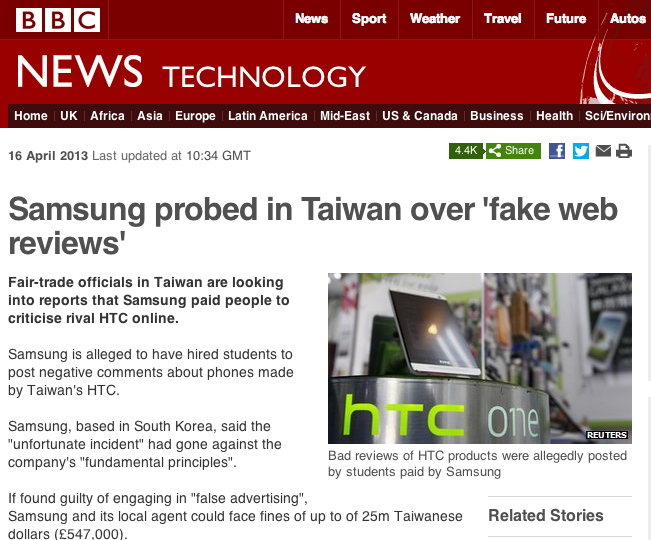
\includegraphics[width=\textwidth]{samsung-spam}
\end{center}

\end{block}


\end{frame}


\begin{frame} \frametitle{Problem is Widespread} %% 169


\begin{block}{\url{http://www.guardian.co.uk/technology/2011/mar/17/us-spy-operation-social-networks}} 

\begin{center}
     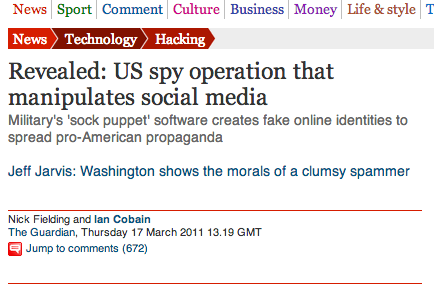
\includegraphics[width=\textwidth]{us-spy-operation}
\end{center}

\end{block}


\end{frame}



\begin{frame} \frametitle{Problem is widespread} %% 169


\begin{block}{\url{http://www.nytimes.com/2004/02/14/us/amazon-glitch-unmasks-war-of-reviewers.html}} 

\begin{center}
     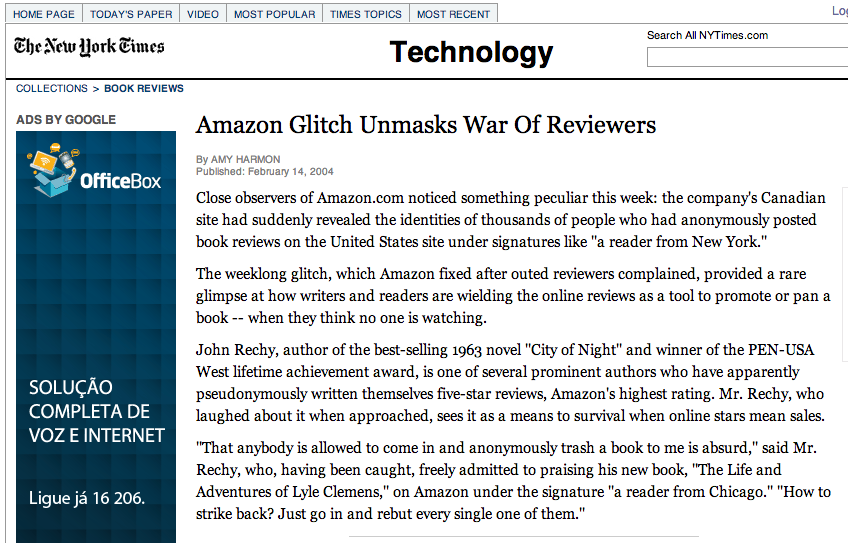
\includegraphics[width=\textwidth]{nytimes-war-reviewers}
\end{center}

\end{block}


\end{frame}



\begin{frame} \frametitle{Problem is Widespread} %% 169


\begin{block}{\url{http://tinyurl.com/cyaga4q}} 

\begin{center}
     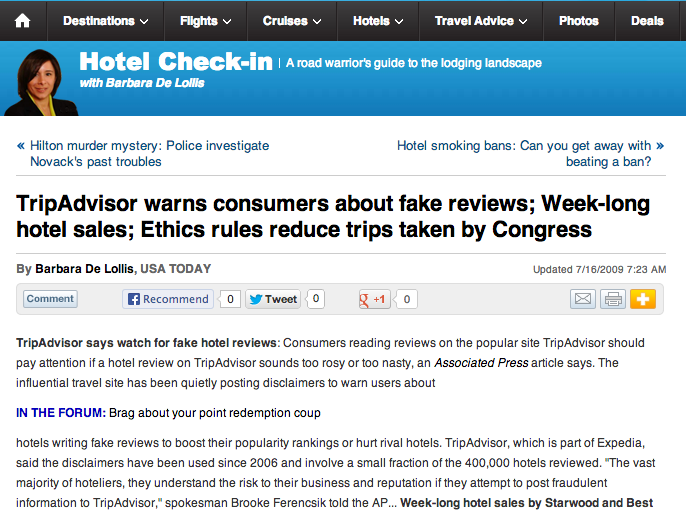
\includegraphics[width=\textwidth]{tripadvisor}
\end{center}

\end{block}


\end{frame}



\begin{frame} \frametitle{Problem is Widespread} %% 169


\begin{block}{\url{https://payperpost.com/}}

\begin{center}
     
\includegraphics[width=\textwidth]{payperpost}
\end{center}

\end{block}


\end{frame}


\begin{frame} \frametitle{Problem is Widespread} %% 170

\begin{block}{http://tinyurl.com/d84axys}

\begin{center}
     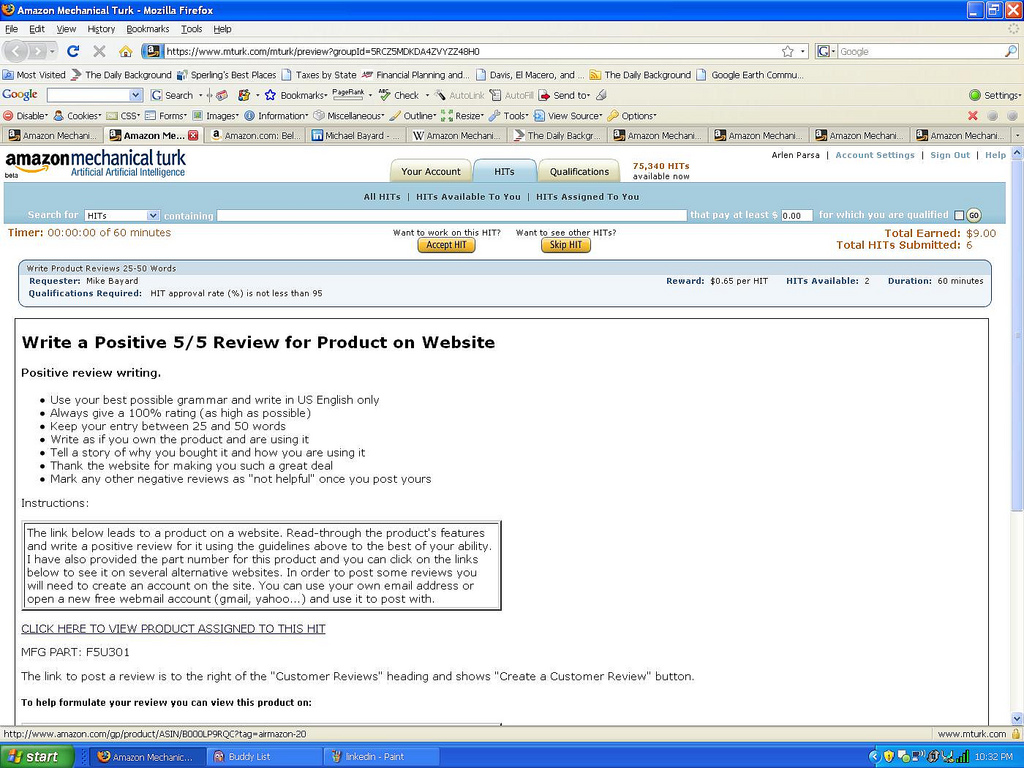
\includegraphics[width=\textwidth]{belkin}
\end{center}

\end{block}

\small{Belkin International, top networking and peripherals manufacture,
posted an ad on Mechanical Turk \url{https://www.mturk.com} for writing fake reviews on Amazon.com (65 cents per
review) Jan 2009
}

\end{frame}

\begin{frame} \frametitle{Power Laws of Amazon Reviews, Reviewers and Products} %% 171

(Jindal and Liu 2008) \\
\url{http://www.cs.uic.edu/~liub/FBS/opinion-spam-WSDM-08.pdf}


\begin{columns}[T]

\begin{column}{0.5\textwidth}

\begin{center}
     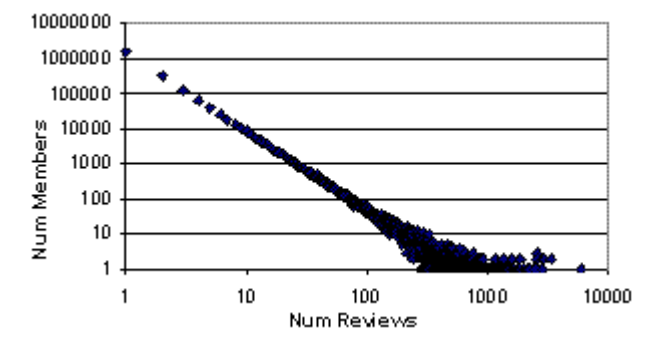
\includegraphics[width=\textwidth]{amazon-reviews-members}
\end{center}
Fig. 1 reviews and reviewers

\end{column}

\begin{column}{0.5\textwidth}

\begin{center}
     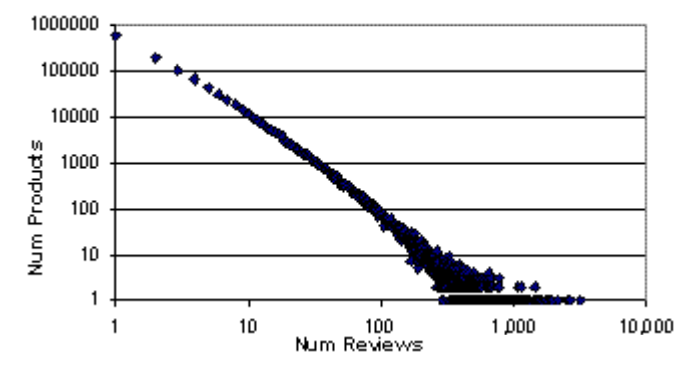
\includegraphics[width=\textwidth]{amazon-reviews-products}
\end{center}
Fig. 2 reviews and products

\end{column}
\end{columns}


%% Fig. 3 reviews and feedbacks


\end{frame}



\begin{frame} \frametitle{Types of Opinion Spam \\ \small{(Jindal and Liu 2008) 
}}  %% 172
  
\textbf{Type 1: Fake Reviews}  \\
\begin{description}
\item [Hype spam:] promote one's own products  
\item [Defaming spam:] defame one's competitors' products
\end{description}

\vfill
\textbf{Type 2: Reviews on Brands Only} \\
Ex: ``I don't trust HP and never bought anything from them''\\
Detectable with a supervised classification method.

\vfill
\textbf{Type 3: Non-reviews} \\
\begin{itemize}
\item Advertisements \\
Ex: ``Detailed product specs: 802.11g, IMR compliant, ...'' ``...buy this product at: compuplus.com''
\item Other non-reviews \\
Ex: ``What port is it for" "The other review is too funny" "Go Eagles go''
\end{itemize}

\end{frame}



%% BL173 can be safely skipped.

\begin{frame} \frametitle{Outlier Reviews as Harmful Spam} %% 174

\begin{block}{Assumption: Most reviewers and reviews are honest}
Not true when a group of people spam on a product, called \textbf{group spam},
discussed next.
\end{block}
\vfill

\textbf{Outlier reviews:} Reviews whose rates deviate significantly from the average product rating 

\vfill
\textbf{Harmful spam reviews:}
\begin{itemize}
 \item Outlier is a necessary but not sufficient condition for harmful spam
reviews. 
\item Helps us identify learning features for opinion spam detection.
\end{itemize}


\end{frame}


\begin{frame} \frametitle{Spam Detection} %%175

Type 2 and Type 3 spam reviews are relatively easy to detect
\begin{itemize} 
\item Supervised learning, e.g. logistic regression, performs quite well
\end{itemize}

Type 1 spam (fake) reviews are harder to detect
\begin{itemize}
\item Manual labeling is extremely hard 
\item Idea: use duplicate and near-duplicate reviews as positive training data
\end{itemize}

\end{frame}



\begin{frame} \frametitle{Duplicate Reviews} %% 176
\textbf{Duplicates:} pairs of reviews with similar content

\vfill
Prevalence in the Amazon dataset:
\begin{center}
     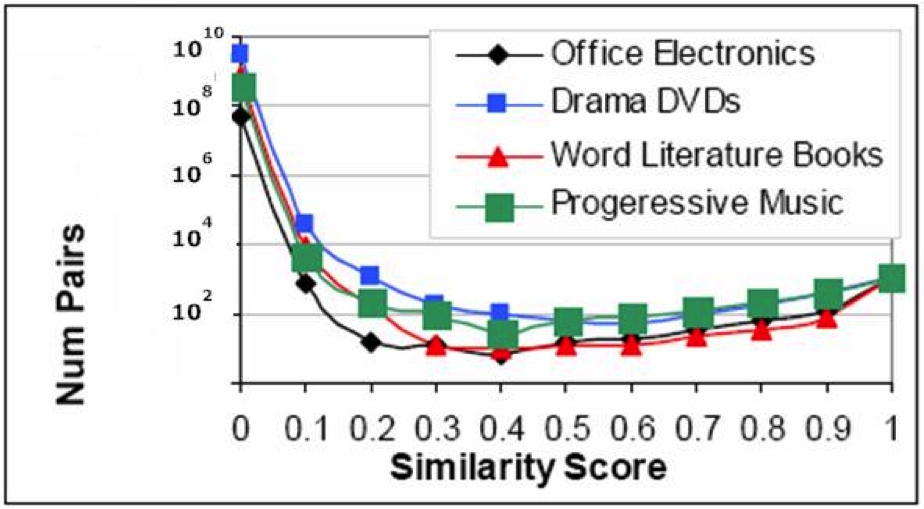
\includegraphics[width=\textwidth]{amazon-reviews-duplicates}
\end{center}

\end{frame}

\begin{frame} \frametitle{Types of Duplicates} %% 177

\begin{enumerate}
\item \textcolor{green}{Same userid, same product }
\item \textcolor{red}{Different userid, same product }
\item \textcolor{red}{Same userid, different products }
\item \textcolor{red}{Different userid, different products }
\end{enumerate}

The last three types are very likely to be fake! \\
The first is very common and not likeley spam! (in the Amazon dataset)
\begin{itemize}
  \item accidental double submission
  \item minor revisions after submission
\end{itemize}

\end{frame}

\begin{comment}

\begin{frame} \frametitle{Supervised Model Building} %% 178

Logistic regression
\begin{itemize}
\item Training: duplicates as spam reviews (positive) and the rest as non-spam reviews (negative)
\item Review centric features (content)
\end{itemize}

Use the following data attributes
\begin{itemize}
\item Reviewer centric features (content): About reviews (contents (n-gram), ratings, etc) 
\item Reviewer centric features: About reviewers (different unusual behaviors, etc) 
\item Product centric features: Features about products reviewed (sales rank, etc)
\end{frame}


\begin{frame} \frametitle{Predictive Power of Duplicates} %% 179
 
Representative of all kinds of spam 

\vfill
Only 3\% duplicates accidental 

\vfill

\begin{block}{Can we use duplicates as Type 1 spam reviews with reasonable predictive power?}
Duplicates as positive examples, rest of the reviews as negative
examples
\end{block}
\end{frame}

\begin{frame} \frametitle{Tentative Classification Results} %% 180

\begin{itemize}
\item Negative outlier reviews tend to be heavily spammed 

\item Reviews that are the only reviews of products are likely to be
spammed 

\item Top-ranked reviewers are more likely to be spammers 

\item Spam reviews can get good helpful feedbacks and non-spam reviews can get bad feedbacks
\end{itemize}

\end{frame}


% http://gizmodo.com/ashley-madison-code-shows-more-women-and-more-bots-1727613924
% http://aventar.eu/2015/08/30/perfis-falsos-de-apoio-a-paf-invadem-facebook/

\begin{frame} \frametitle{Detecting Deceptive Reviews \\ small{(Ott et al  2011)}} %% 181


Detecting deceptive language has been studied in psychology, communication and linguistics
(Newman et al 2003; Zhou, Shi and Zhang 2008; Mihalcea and Strapparava 2009).

Ott et al (2011) used the idea to detect deceptive opinion spam reviews with supervised learning.
 
Manually labeled a dataset Various features on genre, psycholinguistic, n-grams

Yoo and Gretzel (2009) also studied deceptive reviews.

\end{frame}

\begin{frame} \frametitle{Finding Unexpected Reviewer Behavior} %% BL182

Since in general it is hard to manually label spam review for
learning, it is thus difficult to detect fake reviews based on review
contents. 

Lim et al (2010) and Nitin et al (2010) analyze the behavior of
reviewers identifying unusual review patterns which may indicate suspicious behaviors of reviewers.

The problem is formulated as finding unexpected rules and rule groups.

\end{frame}

\begin{comment}

\begin{frame} \frametitle{Spam Behavior Models \\ \smal{(Lim et al 2010})
} %% BL183


Several unusual reviewer behavior models were identified.
\begin{itemize}
\item Targeting products 
\item Targeting groups 
\item General rating deviation 
\item Early rating deviation
\end{itemize}

\vfill
Their scores for each reviewer are then combined to produce the final
spam score. 

\vfill
Ranking and user evaluation

\end{frame}

\end{comment}

\begin{frame} \frametitle{Finding Unexpected Rules} %% BL184

(Jindal, Liu, Lim 2010)

\vfill
\textbf{Unexpected} if, for example, a reviewer wrote all positive reviews on products of a
brand but all negative reviews on a competing brand ...

\vfill

Finding unexpected rules,
\begin{itemize}
\item Data: reviewer-id, brand-id, product-id, and a class. 

\item Mining: class association rule mining 

\item Finding unexpected rules and rule groups, i.e., showing atypical behaviors of reviewers.
\end{itemize}

\begin{block}{}
Rule1: Reviewer-1, brand-1 $\rightarrow$ positive (confid=100\%) \\
Rule2: Reviewer-1, brand-2 $\rightarrow$ negative (confid=100\%)
\end{block}

\end{frame}


\begin{comment}

\begin{frame} \frametitle{The example (cont.)}

\end{frame}

\begin{frame} \frametitle{Confidence Unexpectedness} %% BL 186
Rule: reviewer-1, brand-1  positive [sup = 0.1, conf = 1]  If we find
that on average reviewers give brand-1 only 20\% positive reviews
(expectation), then reviewer-1 is quite unexpected.

Cu (v jk  ci ) =
E (Pr(ci | v jk , v gh )) =

Pr(ci | v jk ) - E (Pr(ci | v jk )) E (Pr(ci | v jk ))
Pr(ci | v jk ) Pr(ci | v gh ) m Pr(cr | v jk ) Pr(cr | v gh ) Pr(cr )
186

Pr(ci )r =1


\end{frame}

\begin{frame} \frametitle{Support Unexpectedness} %% BL 187
Rule: reviewer-1, product-1 -> positive [sup = 5]  

Each reviewer should write only one review on a product and give it a
positive or negative rating (expectation).  
This unexpectedness can detect those reviewers who review the same product multiple times, which is unexpected.

These reviewers are likely to be spammers.

Can be defined probabilistically as well.


\end{frame}


\end{comment}


\begin{frame} \frametitle{Group Spam} %% BL 188


\begin{columns}[T]

\begin{column}{0.7\textwidth}
A group of people, or a single person with multiple ids
(\textit{sockpuppets}), work together to promote or demote a
product. 

\vfill
Such spam can be very harmful as they can take control of sentiment on
a product 
\end{column}

\begin{column}{0.3\textwidth}
\begin{center}
     
\includegraphics[width=0.85\textwidth]{sockpuppet}
\end{center}
\end{column}

\end{columns}

\vfill
Mukherjee et al (2011) propose an algorithm with three steps:
\begin{enumerate}
\item Frequent pattern mining: find groups of people who reviewed a number of products
together. 
\item Extract features characteristic of spammer groups
\item Rank groups based on features with a learning to rank algorithm
\end{enumerate}

% http://www.cs.uic.edu/~liub/publications/WWW-2011-group-review-spam.pdf
% later expanded to
% http://www.cs.uic.edu/~liub/publications/WWW-2012-group-spam-camera-final.pdf

\end{frame}


%\section{Utility or helpfulness of reviews}
%\begin{frame} \frametitle{}
%\end{frame} 

\begin{frame} \frametitle{Summary}

\begin{itemize}
\item Sentiment analysis/opinion mining provides a framework to
  structure meaning extracted from unstructured text. 
  \begin{itemize}
    \item Large data and summarization are crucial.
  \end{itemize}
\item Many problems not attempted or studied. None of the problems attempted is
solved. 
\begin{itemize}
\item It is a fascinating NLP or text mining problem. \\
\item Every sub-problem is highly challenging. But it is also highly restricted (semantically).
\end{itemize}

\item The general NLP is probably too hard, but can we solve this highly restricted problem?

\end{itemize}

\begin{block}{Despite the challenges, applications are flourishing!}
It is useful to every organization and individual. \\
Opinion-based search may become possible.
\end{block}

\end{frame}

\begin{frame} \frametitle{References} %% 198

The main content is from Chapter 11 from the book: \\
B. Liu. Web Data Mining: Exploring Hyperlinks, Contents and Usage
Data. Second Edition, Springer, July 2011. 

A list of references mentioned in parts of this tutorial is available
\small{\url{http://www.cs.uic.edu/~liub/FBS/AAAI-2011-tutorial-references.pdf}}

\vfill
Bing Liu. Sentiment Analysis and Opinion Mining, Morgan \& Claypool
Publishers, May 2012. \small{\url{http://www.cs.uic.edu/~liub/FBS/SentimentAnalysis-and-OpinionMining.pdf}}

\vfill
See also project webpages for some local activities involving opinion mining \\
REACTION \url{http://dmir.inesc-id.pt/project/Reaction} \\
POPSTAR \url{http://dmir.inesc-id.pt/project/POPSTAR} 

\end{frame}




% ------------------------------------------------------------
% ------------------------------------------------------------

\finalframe{Questions?}

\end{document}



